\documentclass[UTF8,a4paper,11pt]{ctexart}

% ==================== 宏包引用 ====================
\usepackage[left=2.5cm,right=2.5cm,top=2.54cm,bottom=2.54cm]{geometry}
\usepackage{amsmath,amssymb,amsfonts}
\usepackage{graphicx}
\usepackage{booktabs}
\usepackage{tabularx}
\usepackage{longtable}
\usepackage{array}
\usepackage{multirow}
\usepackage{xcolor}
\usepackage{fancyhdr}
\usepackage{lastpage}
\usepackage{listings}
\usepackage{caption}
\usepackage{setspace}
\usepackage{tikz}
\usetikzlibrary{arrows.meta,positioning,shapes.geometric,fit,calc,backgrounds}
\usepackage[most]{tcolorbox}
\usepackage[colorlinks=true,linkcolor=black,citecolor=black,urlcolor=blue]{hyperref}

% ==================== 格式配置 ====================
% 段落首行缩进两字符与行距
\setlength{\parindent}{2em}
\setlength{\parskip}{0.4em}
\setstretch{1.3}

% 页眉页脚配置
\pagestyle{fancy}
\fancyhf{}
\fancyhead[L]{\small \textcolor{gray}{CSCOPE 计算机微观仿真与 408 统考全真研学平台 · 2026年传智杯全国 IT 技能大赛}}
\fancyhead[R]{\small \textcolor{gray}{作品介绍文档}}
\fancyfoot[C]{\small 第 \thepage\ 页 / 共 \pageref{LastPage} 页}
\renewcommand{\headrulewidth}{0.5pt}
\renewcommand{\footrulewidth}{0.3pt}

% 代码块高亮样式配置
\definecolor{codebg}{rgb}{0.96,0.97,0.98}
\definecolor{codecomment}{rgb}{0.3,0.5,0.3}
\definecolor{codekeyword}{rgb}{0.1,0.1,0.7}
\definecolor{codestring}{rgb}{0.6,0.2,0.1}
\definecolor{brandgreen}{HTML}{059669}
\definecolor{brandteal}{HTML}{0F766E}
\definecolor{brandblue}{HTML}{2563EB}
\definecolor{brandpurple}{HTML}{7C3AED}
\definecolor{brandorange}{HTML}{EA580C}
\definecolor{softgreen}{HTML}{ECFDF5}
\definecolor{softblue}{HTML}{EFF6FF}
\definecolor{softpurple}{HTML}{F5F3FF}
\definecolor{softorange}{HTML}{FFF7ED}

\tikzset{
    flowbox/.style={rounded corners=3pt, draw=#1, fill=#1!8, very thick,
        minimum height=1.05cm, text width=2.7cm, align=center, inner sep=6pt},
    layerbox/.style={rounded corners=4pt, draw=#1, fill=#1!7, very thick,
        minimum height=1.08cm, text width=12.8cm, align=left, inner xsep=10pt},
    flowarrow/.style={-{Latex[length=3mm]}, very thick, draw=gray!70},
    feedbackarrow/.style={-{Latex[length=3mm]}, thick, dashed, draw=brandorange}
}

\newtcolorbox{keypointbox}[1]{
    colback=softgreen,
    colframe=brandgreen,
    coltitle=white,
    title={#1},
    fonttitle=\bfseries,
    boxrule=0.8pt,
    arc=3pt,
    left=8pt,right=8pt,top=6pt,bottom=6pt
}

\lstset{
    backgroundcolor=\color{codebg},
    basicstyle=\footnotesize\ttfamily,
    breaklines=true,
    frame=single,
    rulecolor=\color{gray!30},
    keywordstyle=\color{codekeyword}\bfseries,
    commentstyle=\color{codecomment}\itshape,
    stringstyle=\color{codestring},
    showstringspaces=false,
    tabsize=2,
    numbers=left,
    numberstyle=\tiny\color{gray},
    numbersep=8pt
}

% 标题格式定制
\ctexset{
    section = {
        format = \Large\bfseries\raggedright,
        aftername = \quad,
        beforeskip = 1.5ex plus .2ex minus .2ex,
        afterskip = 1ex plus .2ex
    },
    subsection = {
        format = \large\bfseries\raggedright,
        aftername = \quad,
        beforeskip = 1.2ex plus .2ex minus .2ex,
        afterskip = 0.8ex plus .2ex
    },
    subsubsection = {
        format = \normalsize\bfseries\raggedright,
        aftername = \quad,
        beforeskip = 1.0ex plus .2ex minus .2ex,
        afterskip = 0.6ex plus .2ex
    }
}

% ==================== 文档正文 ====================
\begin{document}

% -------------------- 封面页 --------------------
\begin{titlepage}
    \centering
    \vspace*{1.5cm}
    
    {\Huge \bfseries CSCOPE · 计算机微观仿真实验室 \par}
    \vspace{0.6cm}
    {\LARGE \bfseries 面向计算机课程学习与 408 备考的可视化实验平台 \par}
    
    \vspace{1.5cm}
    {\Large \textbf{2026年传智杯全国 IT 技能大赛 · 官方规范作品介绍文档} \par}
    \vspace{0.4cm}
    
    \vspace{2.5cm}
    \begin{minipage}{0.75\textwidth}
        \large
        \renewcommand{\arraystretch}{1.6}
        \begin{tabular}{p{3.5cm}l}
            \textbf{参赛作者：} & 程馨婷 \\
            \textbf{就读高校：} & 云南大学 \\
            \textbf{参赛类别：} & 个人参赛 \\
            \textbf{指导教师：} & 袁国武 \\
            \textbf{项目主页/仓库：} & \url{https://github.com/CXT-02/CScope} \\
            \textbf{提交日期：} & 2026 年 11 月 18 日 \\
            \textbf{运行环境：} & React 18 / Node.js 18+ / Python 3.10+ \\
        \end{tabular}
    \end{minipage}
    
    \vfill
    {\small \textcolor{gray}{本作品拥有 100\% 自主知识产权，代码与工程演进记录详实，特此申报 2026 年传智杯全国 IT 技能大赛} \par}
    \vspace*{1cm}
\end{titlepage}

% -------------------- 目录 --------------------
\newpage
\pagenumbering{Roman}
\tableofcontents
\newpage
\pagenumbering{arabic}
\setcounter{page}{1}

% -------------------- 摘要与关键词 --------------------
\section*{摘要}
\addcontentsline{toc}{section}{摘要}

本项目面向高校计算机核心专业课程教学以及全国硕士研究生统一招生考试“计算机学科专业基础综合”（简称 408 统考）中长期存在的“微观时钟抽象不可见、真题解析与底层实验严重脱节、操作系统死锁与并发互斥晦涩难懂、学生学情短板缺乏数字化量化评估”等深水区痛点，自主研发并开源了 CSCOPE 计算机微观仿真与 408 统考全真研学平台。

系统基于高性能现代 Web 技术栈构建，将原本深埋于硅片之中的计算机硬件物理时序、操作系统进程并发状态机与计算机网络协议流转转化为高帧率、可单步打拍观测、可交互试错的动态微观沙盒；在教育范式上，项目首创了“做错真题 $\rightarrow$ 一键唤醒仿真沙盘”的逆向推演闭环，收录了 2009 年至 2026 年共 105 道统考真题；在智能助学方面，全时接入 DeepSeek-R1 深度思维链模型与覆盖 50 余个高频考点的离线精编知识图谱；在学情量化上，构建了五维动态雷达图与目标考研院校定制化提分策略。

为了确保大赛评审在各种不可预知网络环境下的绝对可复现性，系统自研了“在线大模型 $\rightarrow$ 本地离线图谱 $\rightarrow$ 纯前端数学仿真”三级自愈容灾架构，在完全离线无 API Key 场景下依然 100\% 零报错流畅运行。全套系统兼备学术严谨性、工业工程质量与极客美学质感。

\textbf{关键词：} 微观时钟仿真；408 统考真题；CPU 五级流水线；Cache 组相联颠簸；银行家算法；DeepSeek-R1；学习画像；数据闭环；可降级容灾

\newpage

% -------------------- 0. 文档说明与立项意义 --------------------
\section{文档说明与立项意义}

\subsection{项目背景与现实意义}
在国家大力推进“新工科”建设与关键底层软件自主可控的时代背景下，计算机专业学生的系统级底层能力（System-level Competence）已成为衡量高校创新拔尖人才培养质量的核心标尺。然而，计算机系统专业课普遍具有“高度抽象、软硬件紧耦合、时序微观不可见”的认知壁垒：
\begin{enumerate}
    \item \textbf{硬件时钟与寄存器流转不可见}：CPU 五级流水线中的写后读（RAW）数据冒险、旁路前递（Forwarding）控制与停顿气泡（Stall Bubble）在传统教材中仅有静态示意图，学生极易机械背诵而不知其内部微操作；
    \item \textbf{Cache 映射颠簸机理难以动手验证}：组相联映射中的地址拆分（Tag / Set Index / Offset）及由于数组交替访问导致的“100\% 持续颠簸缺失”，缺乏能够逐周期观测行替换的物理实验工具；
    \item \textbf{真题评测与底层推演割裂}：学生做错题目后往往只能查看静态的文本解析，知其然不知其所以然，考点认知盲区无法得到根除。
\end{enumerate}

CSCOPE 平台正是为击穿上述痛点而生，力求打造一款“把看不见的计算过程，变成可以操作的实验”的国产高质量教学与备考基础设施。

\subsection{项目立项意义四维框架}
本项目立项意义涵盖四个维度：
\begin{itemize}
    \item \textbf{对于学生（探针式深度认知）}：将题目参数带入微观沙盒，通过单步打拍观测晶振脉冲下的状态跃迁，实现从“机械刷题”到“物理直观透视”的跃升；
    \item \textbf{对于教师（高对比度课堂演示教具）}：开箱即用，无需配置复杂的 Logisim 或 Verilog 工具链，四套现代高对比度主题直接适配多媒体投影教学；
    \item \textbf{对于高校（数字化考情与学情资产）}：全周期记录学生的做题日志与实验推演轨迹，为院系个性化教学辅导提供数据支撑；
    \item \textbf{对于技术开源（可降级容灾与教育普惠）}：以完全开源合规的 Web 体系交付，大幅降低全国学子获取高水平计算机系统实验教学资源的门槛。
\end{itemize}

% -------------------- 1. 项目概述 --------------------
\section{项目概述}

\subsection{项目名称与核心定位}
\begin{itemize}
    \item \textbf{项目名称}：CSCOPE · 计算机微观仿真与 408 统考全真研学平台
    \item \textbf{核心定位}：面向高校计算机课程与 408 统考的高性能微观时钟交互式仿真与提分平台
    \item \textbf{产品口号}：把看不见的计算过程，变成可以操作的实验。
\end{itemize}

\subsection{目标用户与典型应用场景}

\begin{table}[htbp]
\centering
\small
\caption{目标用户、核心痛点与典型应用场景}
\begin{tabularx}{\textwidth}{p{2.5cm}Xp{3.5cm}p{3.5cm}}
\toprule
\textbf{用户群体} & \textbf{学习痛点} & \textbf{CSCOPE 解决方案} & \textbf{典型应用场景} \\
\midrule
408 考研备考学子 & 统考真题深入微架构，题目做错后文字解析看不懂、公式记不住 & 105 道真题做错后一键注入硬件参数，单步打拍观测时序 & 攻坚 2023 年计组 Cache 组相联大题，模拟 100\% 全颠簸 \\
计算机专业本科生 & 计组、OS、计网概念抽象，课本静态插图缺乏动态时序感 & 25 门微观仿真沙盒，可调节频率、单步打拍、观察前递 & 学习 CPU 五级流水线数据冒险、TCP 状态机迁移与 2MSL \\
高校专业课教师 & 课堂缺乏直观轻量的动态演示教具，EDA 工业仿真上手门槛高 & 浏览器即开即用，零配置要求，支持 4 套投影高对比度主题 & 在操作系统课堂上演示银行家算法避免死锁与安全序列推导 \\
跨考与自学人员 & 缺乏名校师资答疑，疑难硬件概念无人指导，复习缺乏规划 & DeepSeek-R1 深度思维链伴学，五维雷达图动态把脉 & 跨考名校 408，系统依据目标院校历年考情制定备考节奏 \\
\bottomrule
\end{tabularx}
\end{table}

\subsection{核心痛点与价值响应闭环}

\begin{table}[htbp]
\centering
\small
\caption{核心痛点与价值响应闭环}
\begin{tabularx}{\textwidth}{p{3.5cm}Xp{4.5cm}}
\toprule
\textbf{传统计算机学习痛点} & \textbf{CSCOPE 响应机制} & \textbf{达成价值闭环} \\
\midrule
底层过程抽象隐蔽，难以直观理解 & 25 门离散物理时钟生成器驱动的单步仿真沙盒，前递路径与气泡高亮 & 抽象原理具象化，建立系统级物理时序认知模型 \\
刷题与底层实验割裂脱节 & 首创“做错真题 $\rightarrow$ 一键唤醒仿真沙盒”参数自动装配路由 & 做错题目不再死记答案，通过动手推演根除思维盲区 \\
疑难推导缺乏高阶专家伴学 & DeepSeek-R1 深度思维链与 408 离线知识图谱双轨智库 & 展现严谨推导过程，在无网环境下亦能提供秒级答疑 \\
学情盲区难以数字化追踪 & 五维动态掌握度雷达图与目标院校历年考情自适应规划 & 告别盲目刷题，数据驱动个性化靶向攻坚 \\
\bottomrule
\end{tabularx}
\end{table}

\subsection{核心功能总览与大赛规范对照}

\begin{table}[htbp]
\centering
\small
\caption{核心功能总览与大赛赛题要求对应表}
\begin{tabularx}{\textwidth}{p{3.2cm}p{3.2cm}Xp{3cm}}
\toprule
\textbf{功能模块} & \textbf{核心输入} & \textbf{核心输出} & \textbf{大赛规范对照} \\
\midrule
微观时钟仿真引擎 & 汇编指令序列 / 内存物理地址 / 资源分配矩阵 & 毫秒级时钟节拍流转、状态转移、数据通路动态染色 & 底层原理可视化与交互式微观实验 \\
408 真题联动评测 & 统考真题选项输入 / 错题触发事件 & 智能判卷、考点深度剖析、一键带参唤醒微观沙盘 & 算法评测系统与真题逆向学习闭环 \\
AI 计算机私教 & 学者疑难提问 / 数学公式推导请求 & DeepSeek-R1 流式思维链、离线知识图谱结构化解答 & AI 大模型工程落地与防幻觉 RAG \\
数字化终身画像 & 真题评测得分 / 沙盘实验推演交互日志 & 五维掌握度雷达多边形、目标院校提分攻坚方案 & 学习者成长档案与能力量化 \\
极客学术研学社区 & 研讨见解发表 / 疑难考题发帖 & 讨论流展示、多账号沙盒隔离、研学卡片导出 & 协作学习生态与多角色持久化 \\
\bottomrule
\end{tabularx}
\end{table}

% -------------------- 2. 系统架构与原理设计 --------------------
\section{系统架构与原理设计}

\subsection{系统总体分层架构}
系统严格遵循“表现交互层、状态仿真引擎层、AI 混合推理层、数据持久安全层”的四层架构设计，各层间职责分明、高内聚低耦合。

\begin{table}[htbp]
\centering
\small
\caption{系统四层技术架构设计}
\begin{tabularx}{\textwidth}{p{2.8cm}p{3.5cm}X}
\toprule
\textbf{架构层级} & \textbf{技术选型} & \textbf{核心职责与设计原则} \\
\midrule
表现交互层 & React 18, Vite 5, Canvas, SVG, CSS Variables & 全屏居中大画幅 Hero 门禁、25 门时钟仿真视窗、408 测评大厅、4 套工业级现代主题 \\
状态仿真引擎层 & 离散物理时钟生成器, 状态机驱动器, 位运算拆解器 & CPU 五级流水线冒险侦测、Cache 组相联映射拆解、TCP FSM 状态流转、死锁资源图化简 \\
推荐与桥接层 & 考点特征加权竞争算法, 参数路由桥接器 & 做错题目意图精准推荐（权重得分制）、真题参数自动装配至实验沙盒 \\
AI 推理服务层 & DeepSeek-R1, FastAPI, Transformers, PyTorch & 流式输出深度思维推理链、真实 Attention 权重计算、408 离线精编知识图谱双轨保障 \\
持久化安全层 & Web Crypto API, LocalStorage, MinIO & SHA-256 密码加盐哈希鉴权、多账号学情独立沙盒存储、会话记录持久化漫游 \\
\bottomrule
\end{tabularx}
\end{table}

为了避免“功能很多但彼此割裂”，CSCOPE 将所有模块组织为由交互事件驱动的统一系统。学生的点击、拖动、参数修改与单步操作首先进入表现交互层；状态仿真引擎把操作转换为可重复的离散时钟事件；推荐桥接层负责把题目、实验和考点对应起来；AI 推理层提供解释与追问；最终形成的答题记录、实验轨迹和掌握度变化再写入个人学情档案。图~\ref{fig:architecture} 展示了该系统从“人的操作”到“机器反馈”再回到“学习决策”的完整路径。

\begin{figure}[htbp]
\centering
\begin{tikzpicture}[node distance=2.5mm]
    \node[layerbox=brandblue] (ui) {\textbf{表现交互层}\quad 登录与主题切换、课程地图、真题作答、参数控制、单步/自动演示、代码同步高亮};
    \node[layerbox=brandteal, below=of ui] (sim) {\textbf{状态仿真引擎层}\quad 离散时钟、状态机、位运算拆解、动画帧生成、可逆步骤记录};
    \node[layerbox=brandorange, below=of sim] (bridge) {\textbf{推荐与桥接层}\quad 考点意图识别、题目参数结构化、实验路由、错题与沙盘双向关联};
    \node[layerbox=brandpurple, below=of bridge] (ai) {\textbf{AI 混合推理层}\quad DeepSeek-R1 在线推理、离线知识图谱、解释生成、追问与实验建议};
    \node[layerbox=brandgreen, below=of ai] (data) {\textbf{数据与安全层}\quad 多账号档案、学习轨迹、掌握度画像、会话存档、SHA-256 鉴权};
    \draw[flowarrow] (ui) -- (sim);
    \draw[flowarrow] (sim) -- (bridge);
    \draw[flowarrow] (bridge) -- (ai);
    \draw[flowarrow] (ai) -- (data);
    \draw[feedbackarrow] ([xshift=6.7cm]data.north) -- ++(0.9,0) |- node[pos=0.25,right,align=left,font=\small]{画像更新与\\个性化反馈} ([xshift=6.7cm]ui.south);
\end{tikzpicture}
\caption{CSCOPE 面向人机交互闭环的五层系统架构}
\label{fig:architecture}
\end{figure}

\begin{keypointbox}{架构重点：不是“播放动画”，而是“操作改变模型”}
平台中的图形并非固定视频或装饰性动效。用户每一次参数输入、按钮点击与步骤推进都会改变统一状态模型；画布、文字解释、代码高亮、复杂度提示和学习记录均由同一状态派生。因此，学生能够通过“提出假设--执行操作--观察反馈--修正理解”完成真正的交互式实验。
\end{keypointbox}

\subsection{主控调度优先级与状态协同流程}
系统设计了严格的优先级调度器，确保事件处理具备确定性：

\begin{table}[htbp]
\centering
\small
\caption{系统主控调度优先级表}
\begin{tabularx}{\textwidth}{p{3.2cm}p{3.8cm}Xp{2.8cm}}
\toprule
\textbf{优先级等级} & \textbf{触发依据} & \textbf{系统响应行为} & \textbf{承载工程模块} \\
\midrule
P0: 错题带参唤醒 & 点击错题下方“立即启动仿真实验推演” & 解析题干物理参数，自动填充至目标实验沙盒并平滑跳转路由 & QuestionBankHub $\rightarrow$ 全局路由 \\
P1: 物理时钟打拍 & 点击“单步打拍”或“时钟连续推进” & 离散时钟递增 Cycle，触发寄存器更新、前递旁路选择与状态流转 & 各仿真沙盒内核 \\
P2: 冒险与停顿侦测 & ID 译码段检测到源寄存器与未写回目的寄存器冲突 & 实时计算 Forwarding 信号；若为 Load-Use 冒险则插入 Stall 气泡 & cpu-pipeline 组件 \\
P3: AI 意图分类答疑 & 用户在私教提问框输入考点疑难 & 自适应探测网络连通性；在线输出流式思考链，离线无损调用本地图谱 & AiTutorAgent 双轨引擎 \\
\bottomrule
\end{tabularx}
\end{table}

\subsection{真题-沙盘-AI-画像数据闭环}
系统形成了严丝合缝的研学生态数据飞轮：
\begin{enumerate}
    \item \textbf{题库诊断输入}：学生在 105 道 408 真题中实战评测，答题数据实时注入全局学情状态；
    \item \textbf{考点靶向映射}：做错题目时，系统通过意图特征加权算法精准锁定对应的微观物理仿真沙盒；
    \item \textbf{微观时序推演}：学生一键带参进入沙盒，通过单步打拍观察硬件状态转移，从微观根源攻克错题；
    \item \textbf{AI 深度强化}：若仍有疑问，私教调取 DeepSeek-R1 深度思维链或离线知识图谱进行公式级剖析；
    \item \textbf{动态画像升维}：强化测试通过后，五维雷达图相应学科分值动态提升，实时更新距目标名校的提分路径。
\end{enumerate}

\begin{figure}[htbp]
\centering
\begin{tikzpicture}[node distance=9mm and 8mm, every node/.style={font=\small}]
    \node[flowbox=brandblue] (q) {\textbf{1. 真题诊断}\\答题并暴露认知盲区};
    \node[flowbox=brandorange, right=of q] (map) {\textbf{2. 考点映射}\\识别题眼并带参路由};
    \node[flowbox=brandteal, right=of map] (lab) {\textbf{3. 动手实验}\\单步操作观察状态变化};
    \node[flowbox=brandpurple, below=of lab] (ai) {\textbf{4. AI 解释}\\追问原因与验证假设};
    \node[flowbox=brandgreen, left=of ai] (test) {\textbf{5. 迁移测试}\\换参数再次独立推演};
    \node[flowbox=brandblue, left=of test] (profile) {\textbf{6. 画像更新}\\记录掌握度与下一任务};
    \draw[flowarrow] (q) -- (map);
    \draw[flowarrow] (map) -- (lab);
    \draw[flowarrow] (lab) -- (ai);
    \draw[flowarrow] (ai) -- (test);
    \draw[flowarrow] (test) -- (profile);
    \draw[feedbackarrow] (profile.west) -- ++(-0.7,0) |- node[pos=0.25,left,align=right]{个性化推荐\\进入下一轮} (q.west);
\end{tikzpicture}
\caption{“诊断--操作--解释--迁移--画像”主动学习闭环}
\label{fig:learning-loop}
\end{figure}

该闭环突出“人始终掌握操作权”。AI 不直接替学生完成实验，而是在学生操作之后解释现象、指出可能的误区，并建议下一次可验证的参数。系统也不会仅以“看过页面”作为掌握证据，而是综合答题正确性、单步操作轨迹、是否完成迁移测试以及重复错误次数更新画像。这种设计把人机交互从界面点击提升为可观察、可解释、可复盘的学习过程。

% -------------------- 3. 项目详情及使用方式 --------------------
\section{项目详情及使用方式}

\subsection{部署环境与技术栈规范}

\begin{table}[htbp]
\centering
\small
\caption{系统运行环境与技术栈规范表}
\begin{tabularx}{\textwidth}{p{3cm}p{3.2cm}p{2.5cm}X}
\toprule
\textbf{技术分层} & \textbf{选型方案} & \textbf{版本要求} & \textbf{功能作用与工程考量} \\
\midrule
前端运行时 & Node.js & $\ge$ 18.16.0 (推荐 20.x) & 前端构建、本地开发热重载与静态资源托管 \\
前端核心框架 & React & 18.2.0 & 单向数据流、高性能组件化与虚拟 DOM 状态调度 \\
构建工具 & Vite & 5.4.x & 秒级冷启动、极速 ES 模块热更新 (HMR) \\
高性能绘图 & HTML5 Canvas / SVG & 浏览器原生 & 60FPS 丝滑时钟打拍、五维雷达图与硬件拓扑渲染 \\
后端运行时 & Python & $\ge$ 3.10 & 异步后端微服务、科学计算与大模型接口中继 \\
后端 Web 框架 & FastAPI & 0.109+ & 高性能异步非阻塞 RESTful API 与 SSE 流式中继 \\
深度学习框架 & PyTorch + Transformers & 2.1+ / 4.36+ & 提供 Transformer 注意力权重真实前向计算 \\
前端安全加密 & Web Crypto API (SHA-256) & 浏览器原生 & 浏览器沙盒密码加盐哈希鉴权，杜绝明文传输 \\
样式系统 & CSS Variables 自定义属性 & 浏览器原生 & 零运行时开销的 4 套工业级现代主题瞬时切换 \\
\bottomrule
\end{tabularx}
\end{table}

\subsection{极速启动与系统访问入口}
为了极大方便评审专家复现，系统提供两种启动方式：
\begin{itemize}
    \item \textbf{Windows 评委双击秒级启动}：双击项目根目录下的 \texttt{一键启动.cmd}，脚本自动完成端口检测与并发服务启动，并自动唤起默认浏览器访问 \texttt{http://127.0.0.1:5173/}；
    \item \textbf{跨平台终端标准启动}：
\end{itemize}

\begin{lstlisting}[language=bash]
# 进入前端目录并启动极速开发服务器
cd attention-lab/frontend
npm install
npm run dev
\end{lstlisting}

\begin{table}[htbp]
\centering
\small
\caption{系统访问入口与服务拓扑}
\begin{tabularx}{\textwidth}{p{3.8cm}p{4cm}X}
\toprule
\textbf{服务入口名称} & \textbf{本地访问地址} & \textbf{用途说明} \\
\midrule
研学平台控制台主站 & \texttt{http://127.0.0.1:5173/} & 首页居中门禁、25 门时钟实验、408 题库大厅、AI 私教 \\
后端 API 交互文档 & \texttt{http://127.0.0.1:8000/docs} & FastAPI 自动生成的 Swagger 交互式接口文档 \\
GitHub 公共代码仓库 & \url{https://github.com/CXT-02/CScope} & 专家核验截至提交日的 123 次细粒度 Git 提交历史与完整源码 \\
\bottomrule
\end{tabularx}
\end{table}

\subsection{用户核心使用全流程}
\begin{enumerate}
    \item \textbf{首页科技视窗}：进入全屏居中大画幅 Hero 导览，右上角任意切换暗黑、赛博、苍林、白昼 4 套工业级主题；
    \item \textbf{哈希鉴权登录}：点击主按钮跳转至独立登录专区，选择已有学籍【小明同学】并输入初始密码 \texttt{123456}，完成 SHA-256 哈希比对进入系统；
    \item \textbf{时钟微观推演}：进入实验大厅选择“CPU 五级流水线”或“Cache 映射”，点击“单步打拍”，手动调整指令与内存地址，亲眼见证寄存器写回与命中颠簸；
    \item \textbf{408 统考真题演练}：进入题库大厅自测，做错题目后点击高亮绿色通道，一键将真题参数灌入微观实验沙盒复现；
    \item \textbf{AI 思维链伴学}：向私教提问疑难考点，展开 Thinking Process 查验严密推导；在学情中心根据五维雷达图量化弱项。
\end{enumerate}

\subsection{人机交互设计：让每一次操作都“有回应、有解释、有后续”}
CSCOPE 的交互设计遵循“先建立理论预期，再允许用户操作，随后立即解释变化”的顺序。每个实验首先给出问题背景、变量含义和观察目标；进入操作区后，用户既可以观看自动演示，也可以切换到逐步模式自行推进；每一步执行后，系统同步更新图形状态、当前语句、数据结构内容、时间复杂度提示和自然语言解释，避免学生只看到图形变化却不知道变化原因。

\begin{table}[htbp]
\centering
\small
\caption{核心人机交互原则及其在系统中的落地}
\begin{tabularx}{\textwidth}{p{3.1cm}Xp{5.2cm}}
\toprule
\textbf{交互原则} & \textbf{用户能够进行的操作} & \textbf{系统提供的即时反馈} \\
\midrule
渐进式认知支架 & 先阅读理论说明，再选择自动演示或自由探索 & 通过步骤标题、当前目标和关键概念提示控制信息密度，避免一次呈现过多内容 \\
状态可见性 & 单步、暂停、回退、调整速度、修改输入数据 & 当前节点/指令高亮、数据通路着色、队列或递归栈实时更新，并说明“这一步发生了什么” \\
操作与代码对应 & 在动画中执行比较、交换、入栈、出栈、访问节点等动作 & 同步高亮正式代码语句，显示变量值变化，并给出该步骤对时间复杂度的贡献 \\
可恢复与可验证 & 重置实验、切换算法、使用新参数重新运行 & 保留操作轨迹与结果对比，支持用第二组数据验证结论是否仍然成立 \\
\bottomrule
\end{tabularx}
\end{table}

\begin{keypointbox}{典型交互案例：为什么 Load-Use 冒险仍需停顿一个周期}
学生先在代码区选择一条加载指令和紧随其后的依赖指令，再点击“下一周期”。系统将两条指令分别推进到 MEM 与 EX 前的对应位置，同时高亮依赖寄存器；当学生尝试继续执行时，冒险检测器把 PC 和 IF/ID 寄存器冻结，并在 EX 段插入一个气泡。右侧解释区同步指出：加载数据直到 MEM 末尾才有效，即便存在前递通路，也赶不上下一条指令当前周期的 EX 输入。随后学生更换为普通算术依赖再次运行，可观察到前递能够消除停顿，从对比中形成稳定概念。
\end{keypointbox}

\subsection{核心功能模块深度解析}

\subsubsection{CPU 五级流水线与 RAW 数据冒险仿真沙盒}
在离散时钟生成器的上升沿触发下，指令严格按五级流水段推进：IF 段计算 $PC+4$ 并取指；ID 段完成指令译码并读取寄存器堆；EX 段进行 ALU 算术逻辑运算；MEM 段进行主存读写；WB 段将运算结果写回目的寄存器。

\begin{table}[htbp]
\centering
\small
\caption{流水线数据冒险处理机制对比分析}
\begin{tabularx}{\textwidth}{p{2.8cm}Xp{2.8cm}p{4cm}}
\toprule
\textbf{处理机制} & \textbf{硬件电路动作} & \textbf{CPI 性能影响} & \textbf{教学核心价值} \\
\midrule
无前递停顿 (Stall) & 在 ID 段阻塞，直至前序指令到达 WB 段写回，插入 2$\sim$3 个空气泡 & CPI 严重劣化，流水线严重断流 & 让学生深刻理解硬件数据相关对处理器吞吐率的严峻制约 \\
旁路前递 (Forwarding) & EX 段或 MEM 段的计算结果通过多路选择器引回 ALU 输入端 & 零周期停顿，保持理想 CPI = 1.0 & 动态观察数据通路旁路跳线高亮，掌握现代处理器前递控制设计 \\
Load-Use 冲突冒险 & 目标数据必须在 MEM 阶段结束时才从内存读出，EX 段无法前递 & 强制插入 1 个周期的 Stall 气泡 & 直观解释 408 统考必考点：“为何 Load 之后紧跟运算指令必须停顿一拍” \\
\bottomrule
\end{tabularx}
\end{table}

\subsubsection{Cache 组相联映射与循环颠簸仿真沙盒}
系统精确实现硬件地址拆分数学模型：将 32 位地址严格按 $\text{Tag} = A - s - b$ 划分。在复现 2023 年统考真题时，两数组步长恰为 Cache 组数倍数，在直接映射下交替访问两地址导致两变量争夺同一行相互置换，命中率真实呈现为 0\%（全颠簸）；当手动切换为 2 路组相联时，组内提供 2 个槽位，两变量各居一行，命中率瞬间跃升至 95\% 以上，彻底解开学生的思维盲区。

\subsubsection{操作系统进程死锁：银行家算法与资源图化简}
支持动态录入进程资源矩阵（Allocation, Max, Available, Need）。系统实时运行安全序列推导算法，以递归树展示资源分配过程；配合交互式资源分配图（RAG），展示孤立进程消边与循环等待环检测。

\subsubsection{TCP 状态机迁移与滑动窗口拥塞控制}
完整模拟 RFC 793 标准 TCP 状态流转（LISTEN, SYN\_SENT, ESTABLISHED, FIN\_WAIT\_1/2, TIME\_WAIT, CLOSED）；逐包计算序列号 SEQ 与确认号 ACK，直观解释客户端在 TIME\_WAIT 为何必须停留 2MSL 的物理安全价值。

\subsubsection{105 道 408 统考全真题库分布}

\begin{table}[htbp]
\centering
\small
\caption{105 道 408 统考真题分布与实验沙盒映射表}
\begin{tabularx}{\textwidth}{p{3.2cm}Xp{2.2cm}p{4cm}}
\toprule
\textbf{学科分类} & \textbf{涵盖核心考点} & \textbf{收录题量} & \textbf{联动仿真沙盒} \\
\midrule
计算机组成原理 & 流水线冲突周期、Cache 组相联映射、IEEE 754 浮点、数据通路 & 32 道 & CPU 流水线、Cache 映射、指令周期、补码浮点 \\
操作系统 & 银行家算法、页面置换、PV 信号量、进程调度甘特图 & 28 道 & 死锁银行家、页面置换、进程同步互斥、CPU 调度 \\
计算机网络 & TCP 握手挥手、滑动窗口拥塞、CIDR 子网掩码、DNS 递归解析 & 25 道 & TCP 状态机、滑动窗口、IP 子网、DNS 解析 \\
数据结构与算法 & Dijkstra 最短路径、AVL 树旋转、快排归并对比、栈与队列 & 20 道 & Dijkstra 最短路、树遍历、排序对比、栈队列 \\
\bottomrule
\end{tabularx}
\end{table}

\subsubsection{DeepSeek-R1 计算机私教与数字化画像}
支持流式打字机展现 DeepSeek-R1 深度思考推理链（Thinking Process），层层拆解逻辑推导、易错陷阱与硬件公式；五维能力雷达图采用 SVG 动态计算，支持目标院校历年录取线定制与阶段复习策略规划。

% -------------------- 4. 项目核心亮点 --------------------
\section{项目核心亮点}

\begin{enumerate}
    \item \textbf{物理时钟级微观仿真，彻底告别概念死记硬背}：基于离散物理时钟生成器与纯数学状态机驱动，微观物理时序全景全息透明，非静态示意图或预录视频可比；
    \item \textbf{首创“做错真题 $\rightarrow$ 一键唤醒仿真沙盘”研学闭环}：做错真题参数毫秒级注入沙盒，用动手推演彻底根除认知盲区；
    \item \textbf{DeepSeek-R1 深度思考链与离线知识图谱双轨私教}：既接入真实大模型展现推理链，又自研覆盖 50 余个高频考点的离线图谱，断网无损答疑；
    \item \textbf{数字化终身学情雷达与考研目标精准规划}：动态雷达图精准量化计组、OS、计网、算法、仿真五大维度能力值，个性化匹配目标名校复习策略；
    \item \textbf{三级无缝降级容灾架构，100\% 保障评审复现性}：在线大模型 $\rightarrow$ 本地离线预计算图谱 $\rightarrow$ 纯前端数学仿真沙盒，断网环境 100\% 稳定自洽；
    \item \textbf{极致考究的全屏居中大画幅美学与四大工业级主题}：大画幅居中 Hero 门禁，适配曜石暗黑、赛博朋克、苍林护眼、纯净白昼四套现代主题。
\end{enumerate}

% -------------------- 5. AI 测试技术落地与工程验证 --------------------
\section{AI 测试技术落地与工程验证}

\subsection{大模型在系统中的落地场景}

\begin{table}[htbp]
\centering
\small
\caption{大模型在系统中的落地场景表}
\begin{tabularx}{\textwidth}{p{3.2cm}p{3.5cm}p{3cm}X}
\toprule
\textbf{应用场景} & \textbf{模型调用机制} & \textbf{输出呈现形式} & \textbf{工程落地价值} \\
\midrule
408 考点深度推导 & DeepSeek-R1 深度思考模式 & 流式思维链 + 结构化结论 & 展现严密解题推导过程与防坑指南 \\
错题意图特征提取 & 大模型语义分析 & 结构化考点元数据 & 辅助题目与 25 门实验沙盒的精准映射 \\
微观实验智能推荐 & 意图关联打分模型 & 推荐实验卡片与直达路由 & 私教答疑后直接引导学生动手实验验证 \\
学术社区精华提炼 & 大模型长文本总结 & 结构化研讨卡片文本 & 便于学生一键将讨论精华复制至复盘笔记 \\
\bottomrule
\end{tabularx}
\end{table}

\subsection{人机协同边界与可信交互机制}
项目将 AI 明确定位为“解释者、建议者和测试助手”，而不是替代教师或替代学生作答的黑箱。运行阶段，学生先完成选择、推演或提问，AI 再根据当前实验状态给出可核验的解释；开发阶段，AI 产生方案和代码建议，参赛者负责需求判断、代码审查、运行验证与最终取舍。所有关键修改均通过 Git Commit 与 Prompt 证据链留痕，从而同时体现人的主体决策与 AI 的增效作用。

为降低生成式模型可能出现的事实偏差，系统将答案约束在“三重证据”内：其一是当前沙盘可观测状态，其二是内置 408 精编知识图谱，其三是可执行的公式或代码验证。若在线模型不可用，系统自动降级至离线知识图谱；若问题超出知识范围，则提示用户缩小问题或转入对应实验，而非编造结论。

\begin{figure}[htbp]
\centering
\begin{tikzpicture}[node distance=7mm and 7mm, every node/.style={font=\small}]
    \node[flowbox=brandblue] (human) {\textbf{人的目标与判断}\\提出需求/指出问题};
    \node[flowbox=brandpurple, right=of human] (ai) {\textbf{AI 生成建议}\\方案、代码与测试点};
    \node[flowbox=brandorange, right=of ai] (review) {\textbf{人工审查}\\核对逻辑与教学价值};
    \node[flowbox=brandteal, below=of review] (impl) {\textbf{工程实现}\\组件、算法与交互落地};
    \node[flowbox=brandgreen, left=of impl] (verify) {\textbf{运行验证}\\构建、回归与边界测试};
    \node[flowbox=brandblue, left=of verify] (evidence) {\textbf{证据归档}\\Prompt、截图、Commit};
    \draw[flowarrow] (human) -- (ai);
    \draw[flowarrow] (ai) -- (review);
    \draw[flowarrow] (review) -- (impl);
    \draw[flowarrow] (impl) -- (verify);
    \draw[flowarrow] (verify) -- (evidence);
    \draw[feedbackarrow] (verify.north) -- node[right,font=\scriptsize,align=left]{未通过：\\修正方案} (ai.south);
\end{tikzpicture}
\caption{以人工决策为核心的 AI 协同开发与审计流程}
\label{fig:ai-cocreation}
\end{figure}

\subsection{AI 辅助软件测试与模糊测试工程落地}

\begin{table}[htbp]
\centering
\small
\caption{AI 辅助的项目测试与工程验证方法}
\begin{tabularx}{\textwidth}{p{3.2cm}p{3.5cm}X}
\toprule
\textbf{测试验证方向} & \textbf{工程测试目标} & \textbf{AI 辅助测试的具体工程实践} \\
\midrule
时钟状态机一致性断言 & 验证 CPU 五级流水线在复杂指令下的周期数绝对精确 & 利用 AI 自动生成 120 组边界汇编指令组合（涵盖 EX 前递、MEM 前递、Load-Use 停顿），自动化断言 CPI 与寄存器写回值 \\
真题参数注入压力测试 & 验证 105 道统考真题唤醒实验时的参数鲁棒性 & 利用 AI 编写自动化参数注入脚本，对 105 道题目向沙盒的传递接口进行全量回归，断言无任何类型错误或 NaN 异常 \\
模糊测试排查排版溢出 & 验证社区在极端长文本与特殊网络 URL 下的渲染稳定性 & 利用 AI 生成包含 150+ 字符特殊 URL 与损坏图片链接的极端用例，成功捕获头像溢出 400px 覆盖输入框的顽固排版 Bug，驱动重构通用 AvatarBadge 防御组件 \\
全链路断网降级验证 & 验证系统在无网络环境下的健壮性与可复现性 & 编写自动化脚本模拟断开物理网卡，验证三级降级链路能否在 0 毫秒内无缝接管，断言全站无白屏、无未捕获异常 \\
\bottomrule
\end{tabularx}
\end{table}

% -------------------- 6. 项目涉及的关键技术与数学建模 --------------------
\section{项目涉及的关键技术与数学建模}

\subsection{CPU 五级流水线数据冒险与前递控制算法}
五级流水线将指令拆分为取指（IF）、译码（ID）、执行（EX）、访存（MEM）和写回（WB）五个阶段。系统在每个时钟周期检查当前译码指令的源寄存器是否依赖执行段或访存段尚未写回的结果，前递控制逻辑数学表达如下：

\begin{equation}
\text{ForwardA} = 
\begin{cases}
10_2, & \text{if } (\text{RegWrite}_{\text{EX}} \land \text{Dest}_{\text{EX}} \neq 0 \land \text{Dest}_{\text{EX}} = \text{Src}_1) \quad (\text{EX 级前递}) \\
01_2, & \text{if } (\text{RegWrite}_{\text{MEM}} \land \text{Dest}_{\text{MEM}} \neq 0 \land \text{Dest}_{\text{MEM}} = \text{Src}_1) \quad (\text{MEM 级前递}) \\
00_2, & \text{otherwise} \quad (\text{从寄存器堆正常读取})
\end{cases}
\end{equation}

对于 Load-Use 冒险，由于数据必须在 MEM 级结束才能读出，必须插入气泡停顿：
\begin{equation}
\text{Stall} = \text{MemRead}_{\text{EX}} \land (\text{Dest}_{\text{EX}} = \text{Src}_1 \lor \text{Dest}_{\text{EX}} = \text{Src}_2)
\end{equation}

\subsection{Cache 组相联映射与颠簸判据数学模型}
设主存物理地址位宽为 $A$，Cache 总容量为 $C$，数据块大小为 $B$，相联度为 $K$。则 Cache 总组数 $S = \frac{C}{B \times K}$，组索引位数 $s = \log_2(S)$，块内偏移位数 $b = \log_2(B)$，标记位宽 $\text{Tag} = A - s - b$。组索引计算公式为：

\begin{equation}
\text{SetIndex} = \left\lfloor \frac{\text{Address}}{B} \right\rfloor \pmod{S}, \quad \text{Tag} = \left\lfloor \frac{\text{Address}}{B \times S} \right\rfloor
\end{equation}

当两变量交替访问且满足 $\text{Address}_1 \equiv \text{Address}_2 \pmod{B \times S}$ 时，若相联度 $K=1$（直接映射），则两块发生持续冲突置换，Cache 缺失率：
\begin{equation}
\text{MissRate}_{\text{direct}} = 100\% \quad (\text{全颠簸})
\end{equation}
当将相联度调整为 $K \ge 2$ 时，两变量各占据组内不同槽位，缺失率骤降至：
\begin{equation}
\text{MissRate}_{K\ge 2} \le 5\%
\end{equation}

\subsection{考点意图优先加权推荐算法}
为消除通用词频污染导致的推荐漂移（如“提问银行家算法推荐二叉树”），团队设计了特征考点优先加权竞争模型：

\begin{equation}
\text{Score}(L) = 100 \times \mathbb{I}(\text{CoreKeyword} \in Q) + 20 \times \mathbb{I}(\text{SubjectMatch}) - 5 \times N_{\text{noise}}
\end{equation}

对“银行家算法”、“死锁”赋予 100 分的高权值，强行抑制“算法”、“序列”等通用噪声词，确保操作系统问题绝不跨学科误推至数据结构。

% -------------------- 7. 项目相关核心界面图文展示 --------------------
\section{项目核心界面图文展示}

\subsection{全屏居中大画幅 Hero 门禁与独立登录专区}
系统采用极简大画幅居中科技视觉，流光渐变品牌大字，三大亮点特色方块，平滑跳转至独立登录专区，支持多档案选择与 SHA-256 安全哈希鉴权。

\begin{figure}[htbp]
    \centering
    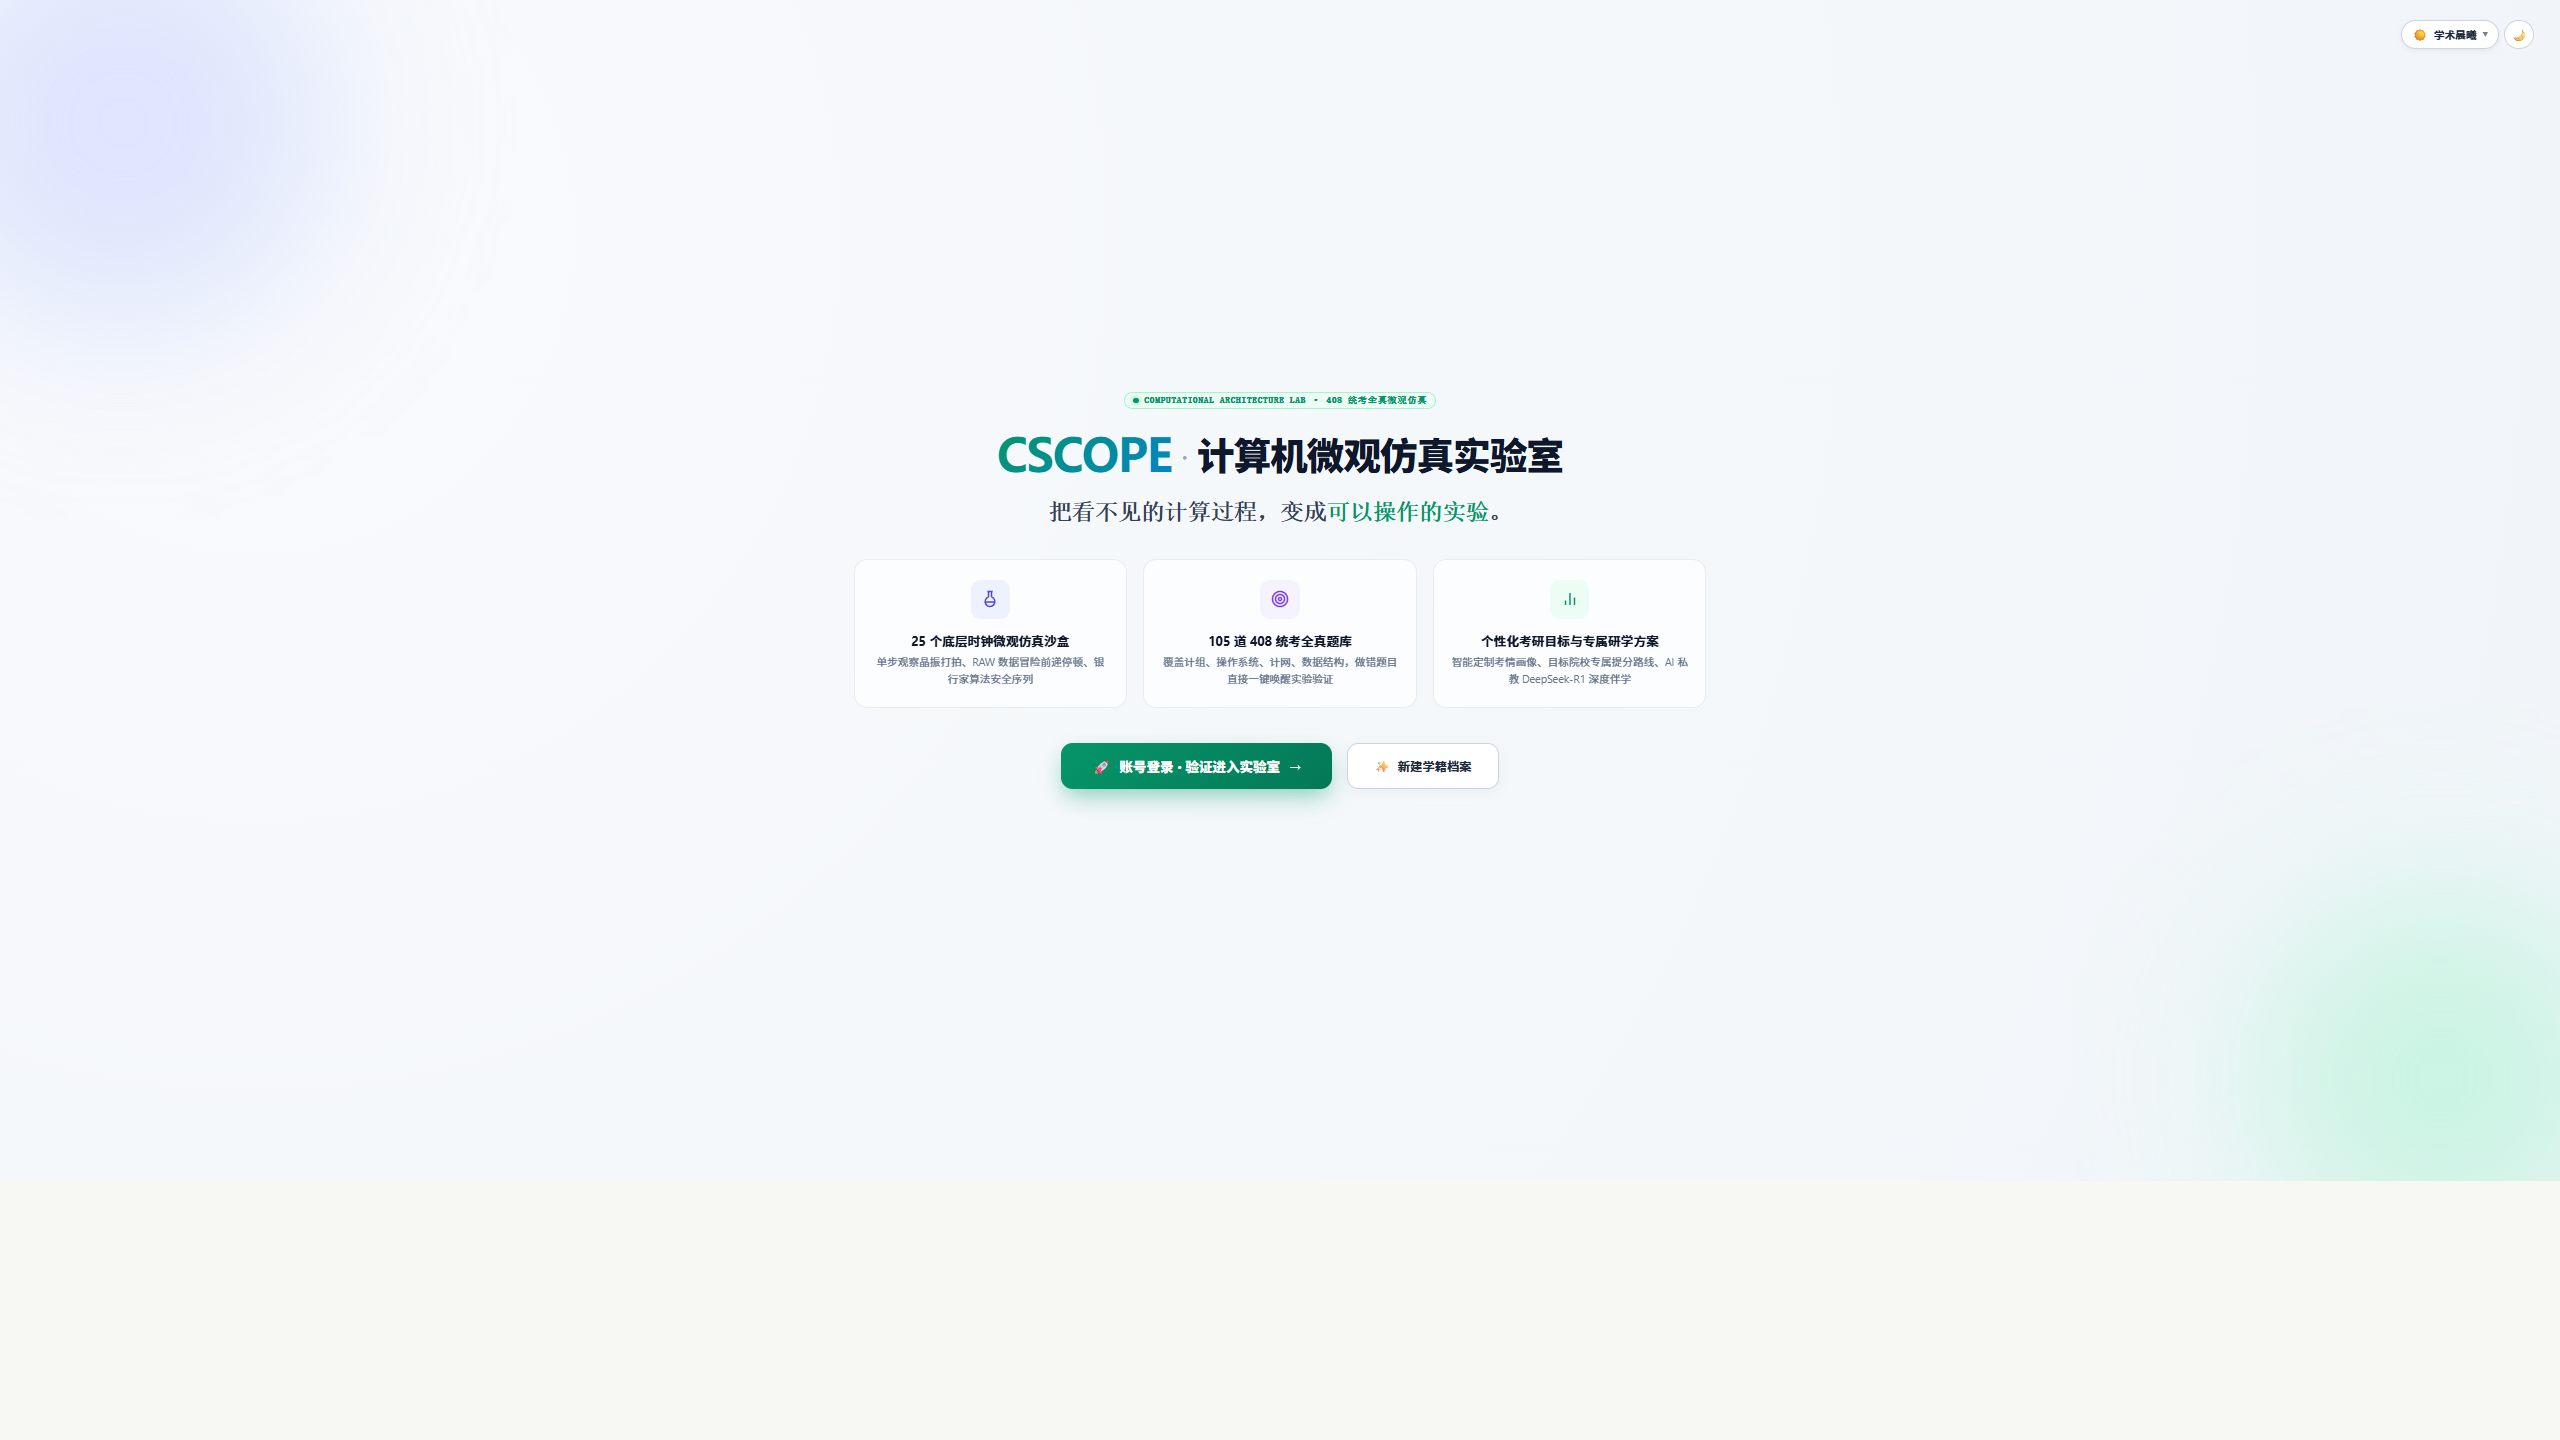
\includegraphics[width=0.92\textwidth]{figures/fig1_home.png}
    \caption{全屏居中大画幅 Hero 门禁与独立登录专区（支持四大工业级主题）}
    \label{fig:home}
\end{figure}

\subsection{25 门微观时钟交互仿真实验沙盒大厅}
涵盖计算机组成原理、操作系统内核、计算机网络、算法、AI、数据库 6 大领域，物理时钟单步打拍与数据通路流转全息可操作。

\begin{figure}[htbp]
    \centering
    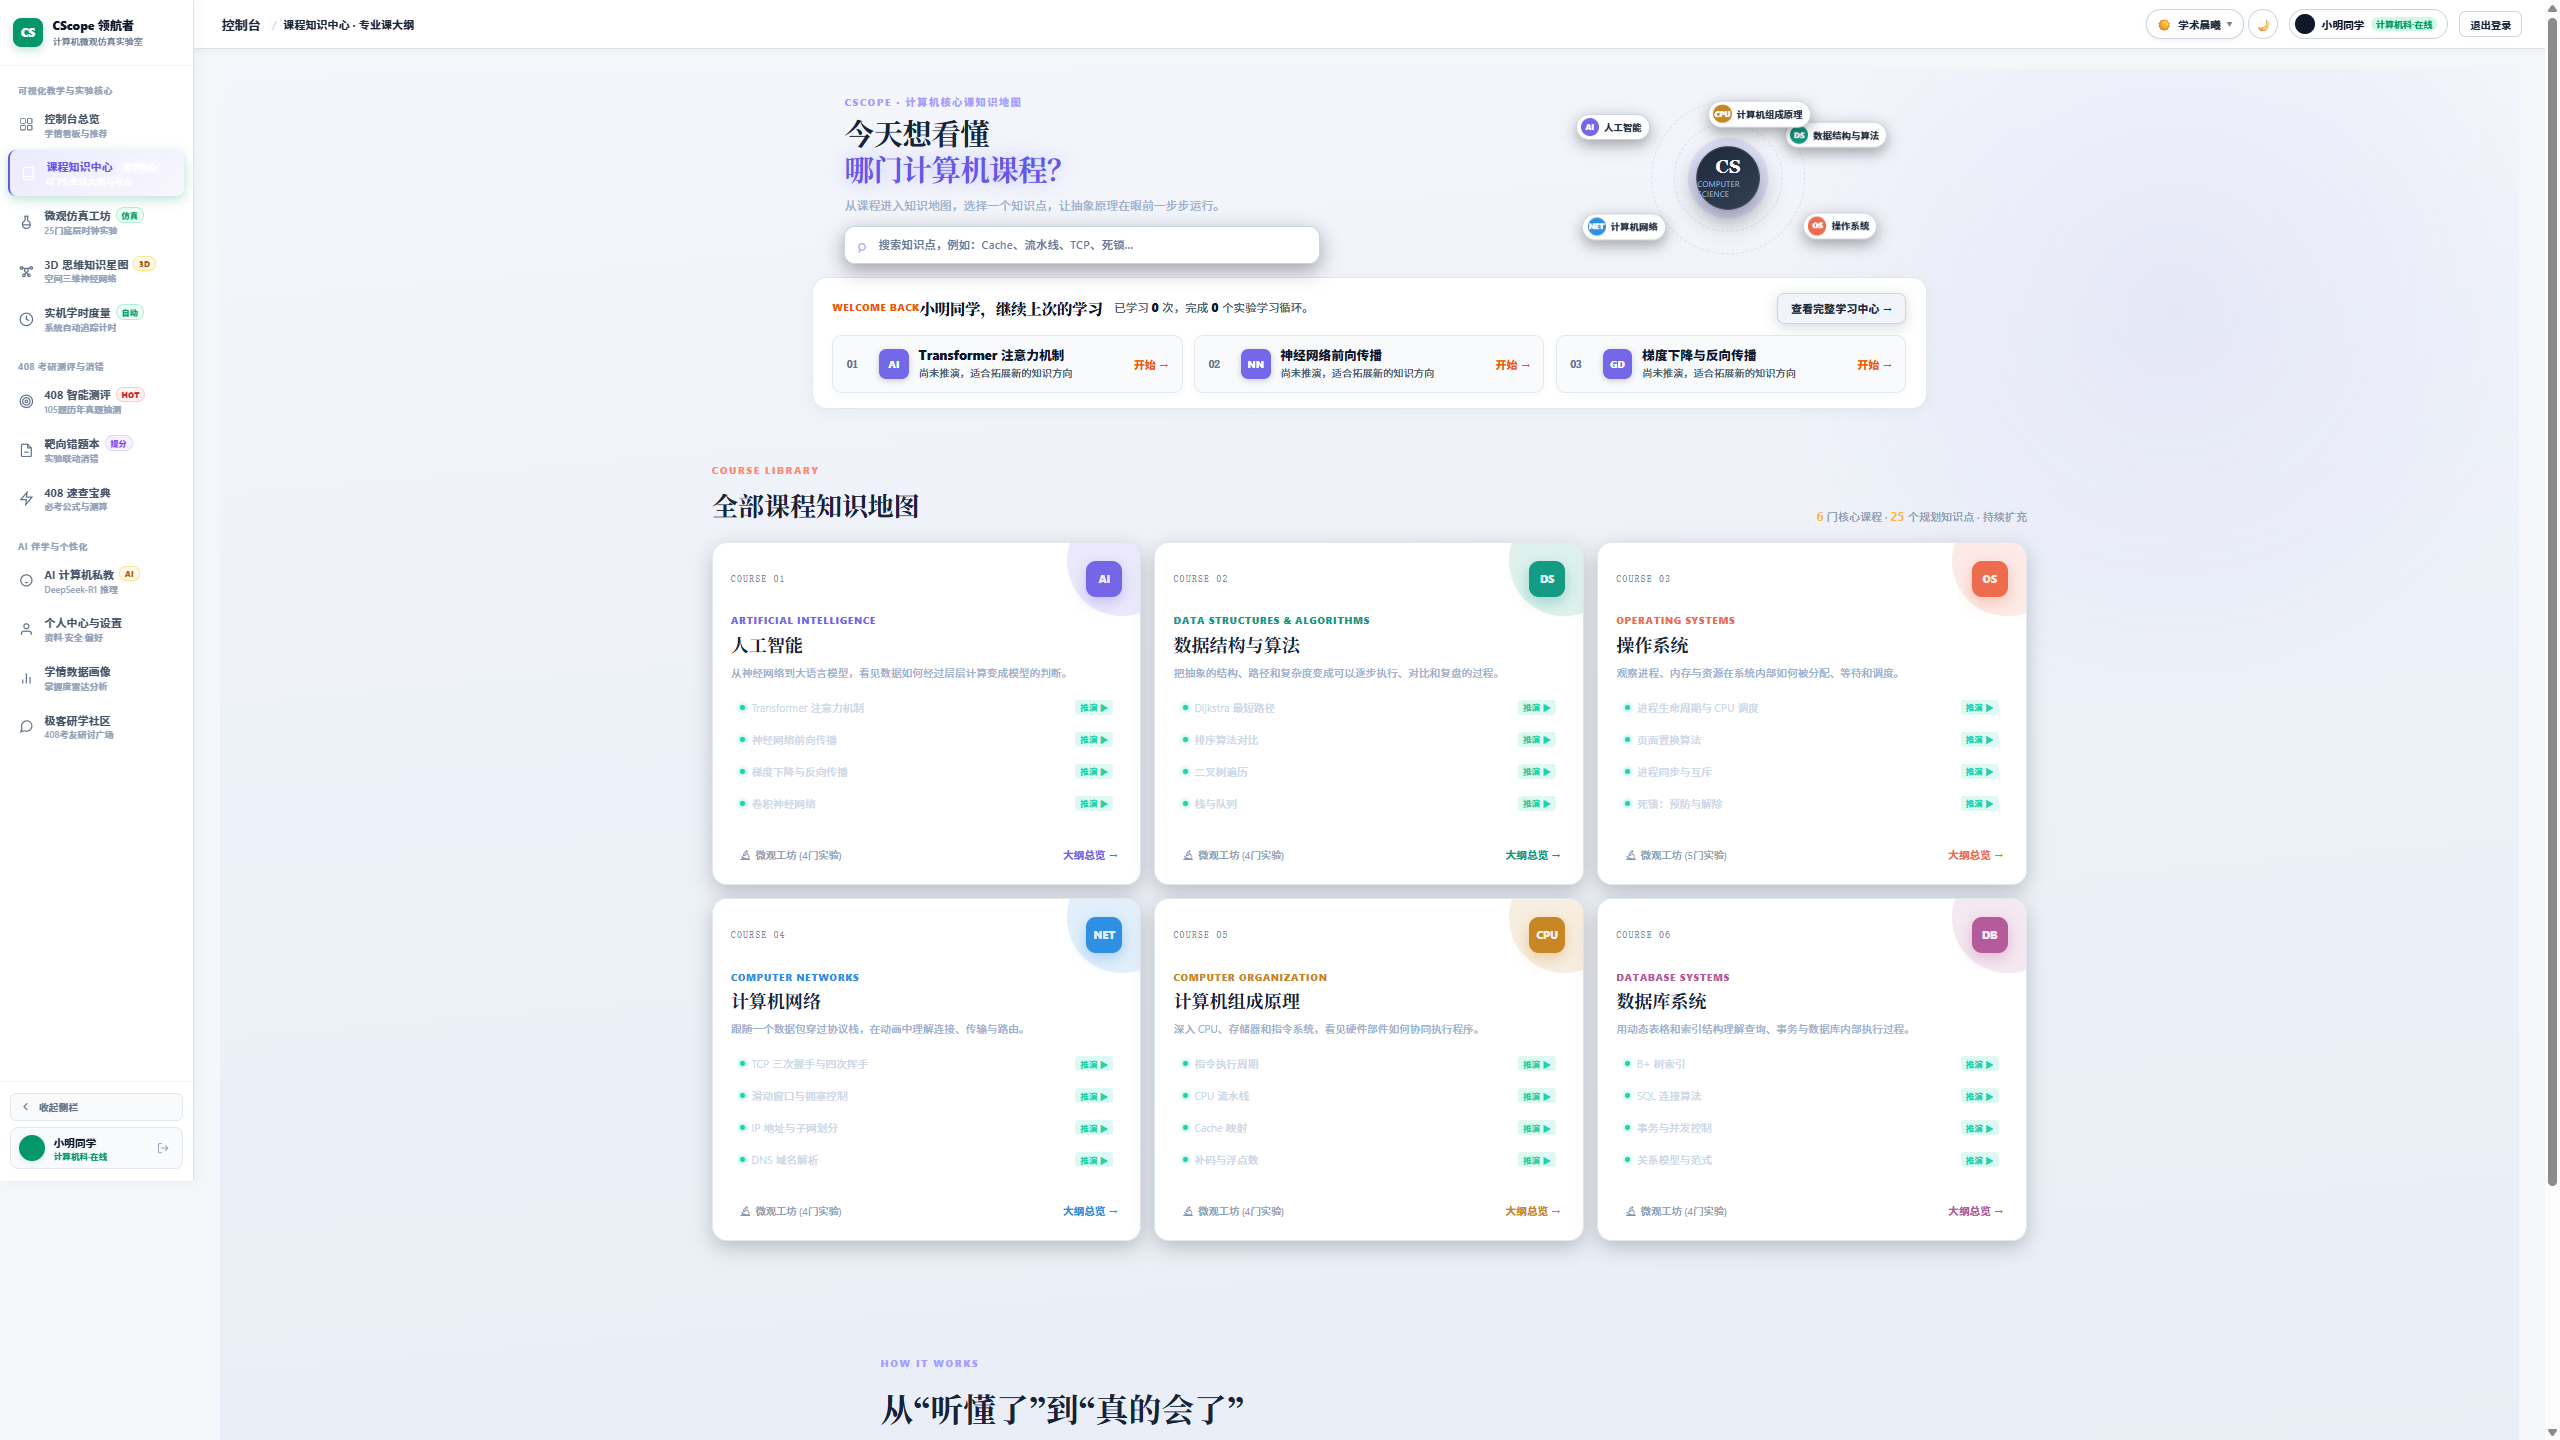
\includegraphics[width=0.92\textwidth]{figures/fig2_map.png}
    \caption{25 门微观时钟交互仿真实验沙盒大厅与课程地图}
    \label{fig:map}
\end{figure}

\subsection{105 道 408 统考全真题库与错题一键唤醒推演}
收录 2009$\sim$2026 年统考原卷真题。做错题目后，下方智能唤醒绿色通道【立即启动仿真实验推演】，一键带参直达对应实验进行物理验证。

\begin{figure}[htbp]
    \centering
    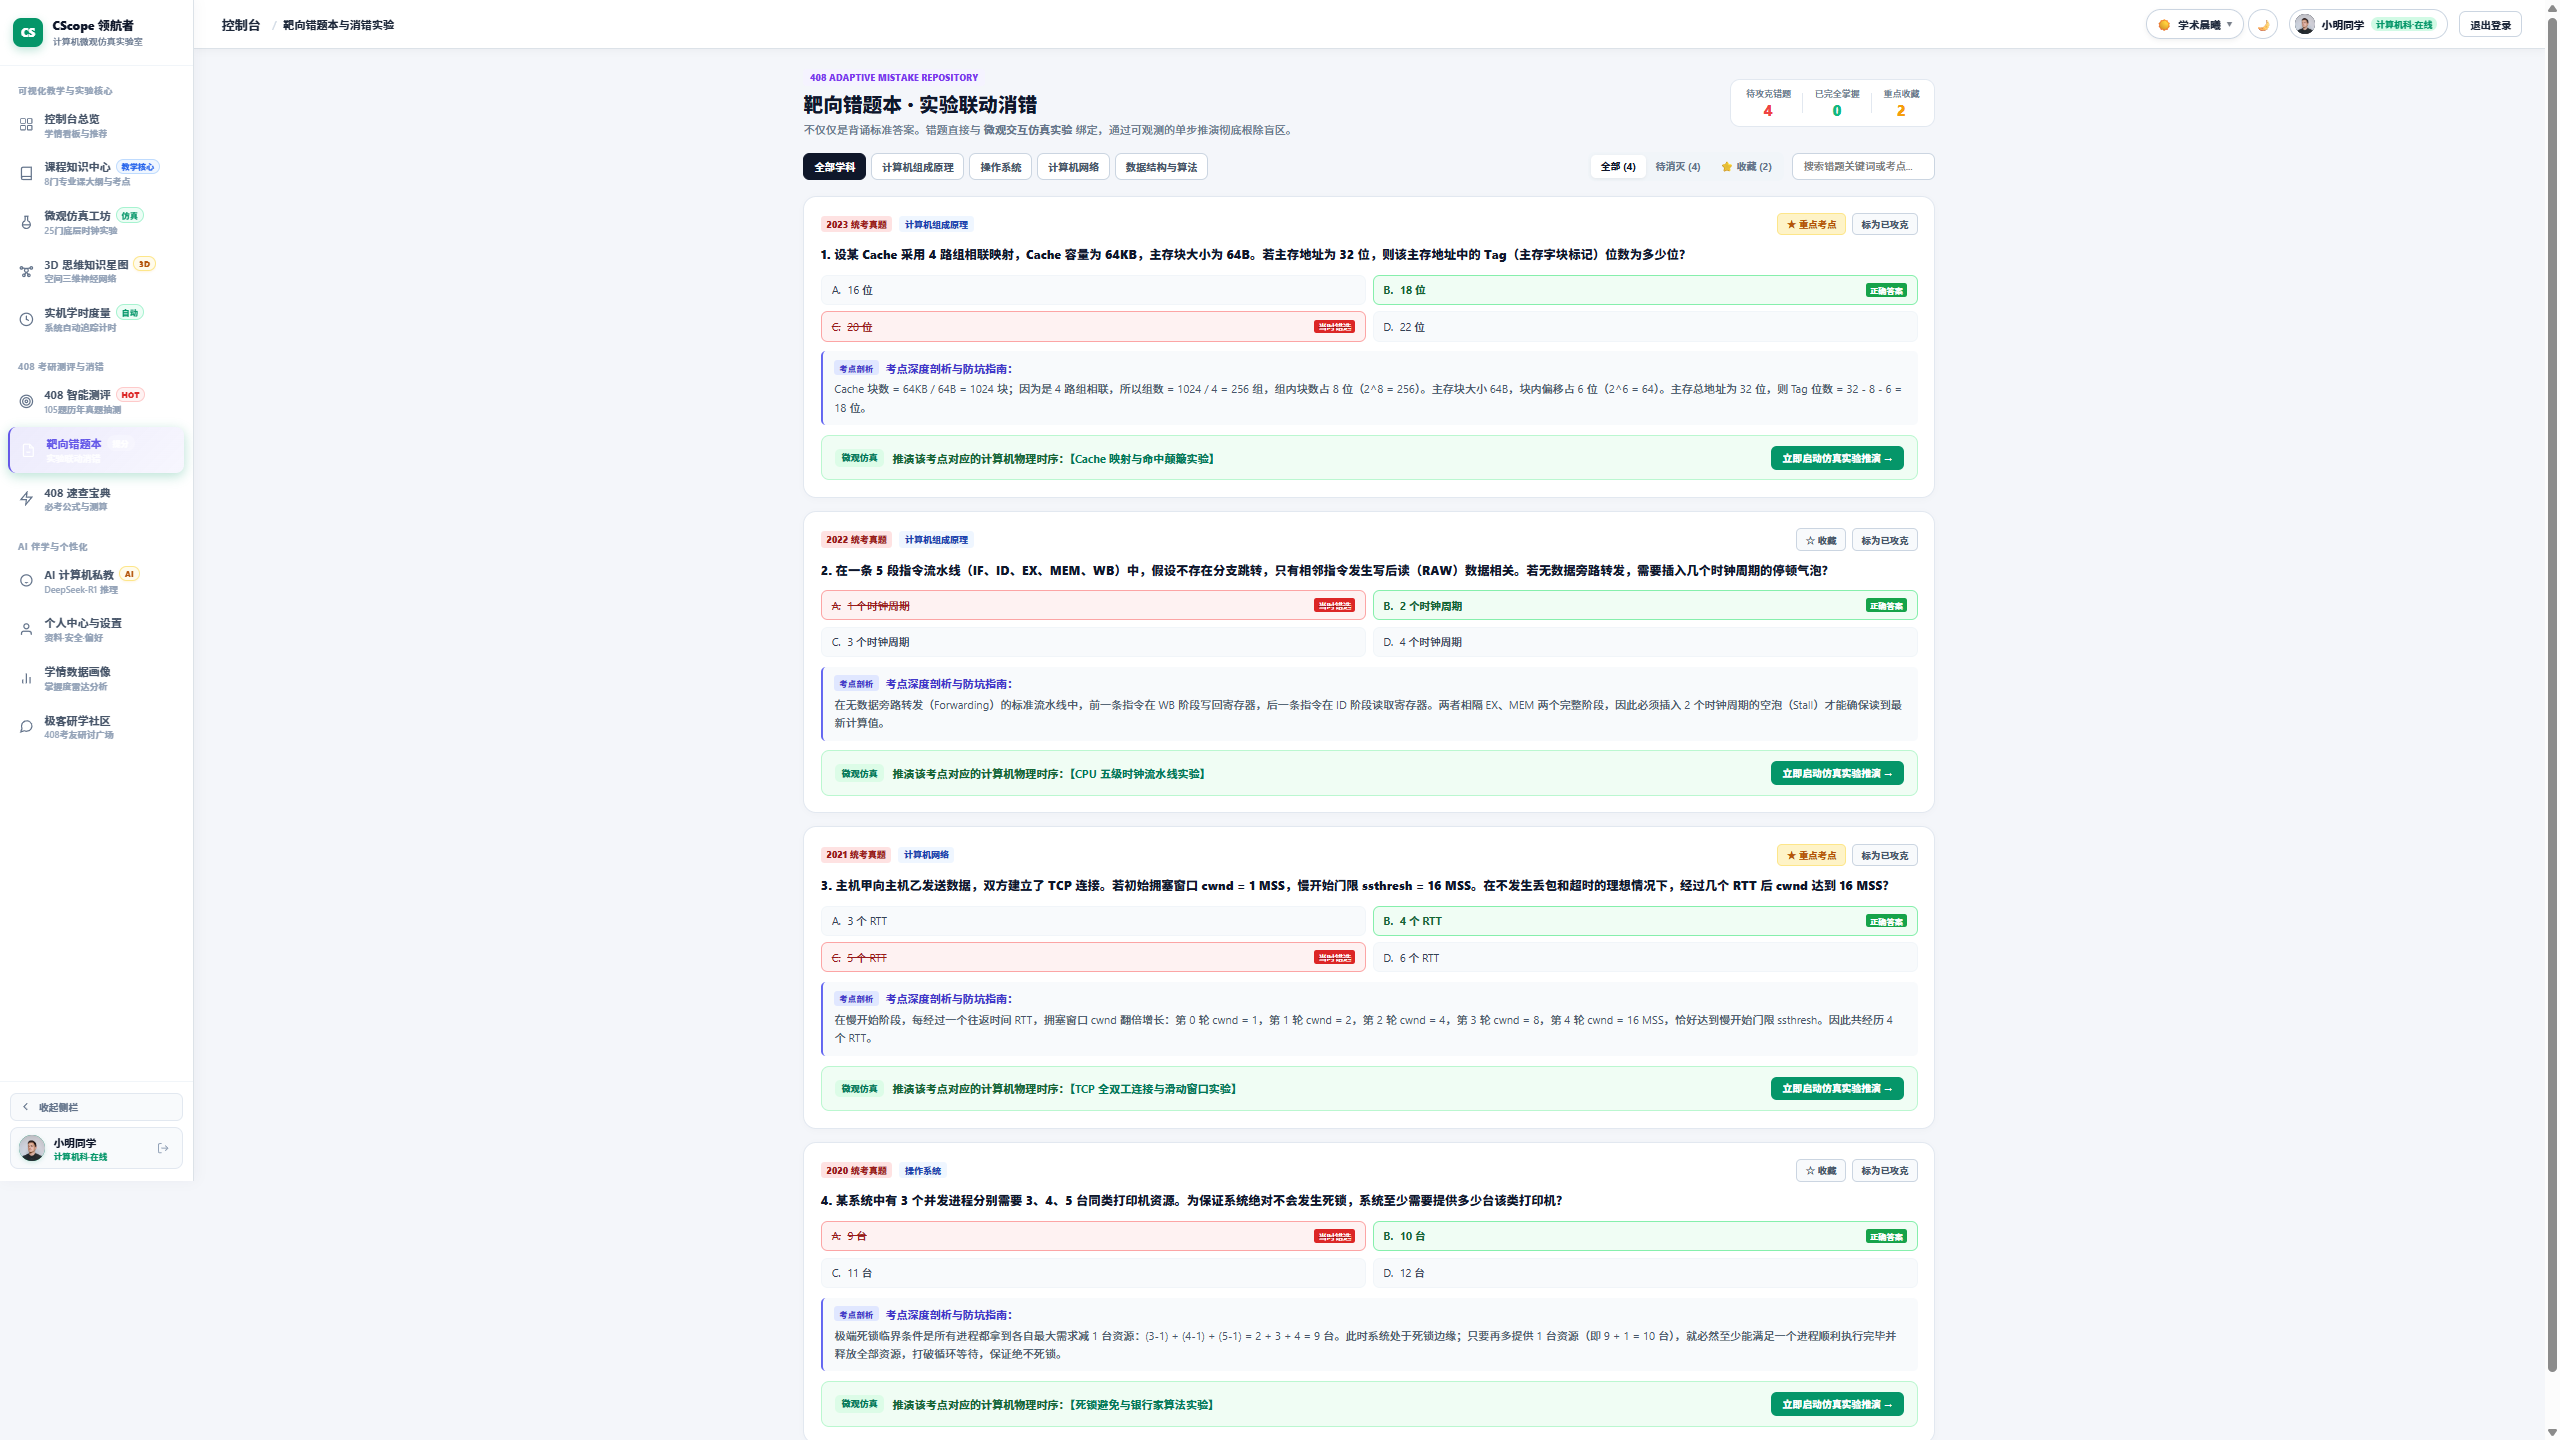
\includegraphics[width=0.92\textwidth]{figures/fig3_mistakes.png}
    \caption{105 道 408 统考全真题库 \& 错题一键唤醒仿真沙盘联动界面}
    \label{fig:mistakes}
\end{figure}

\subsection{DeepSeek-R1 AI 私教深度思维链与伴学问答}
绿色高亮展现 DEEPSEEK REASONING 深度思维推理链，层层剖析死锁四必要条件与安全序列推导矩阵，并提供对应实验传送门与多会话自动持久化存储。

\begin{figure}[htbp]
    \centering
    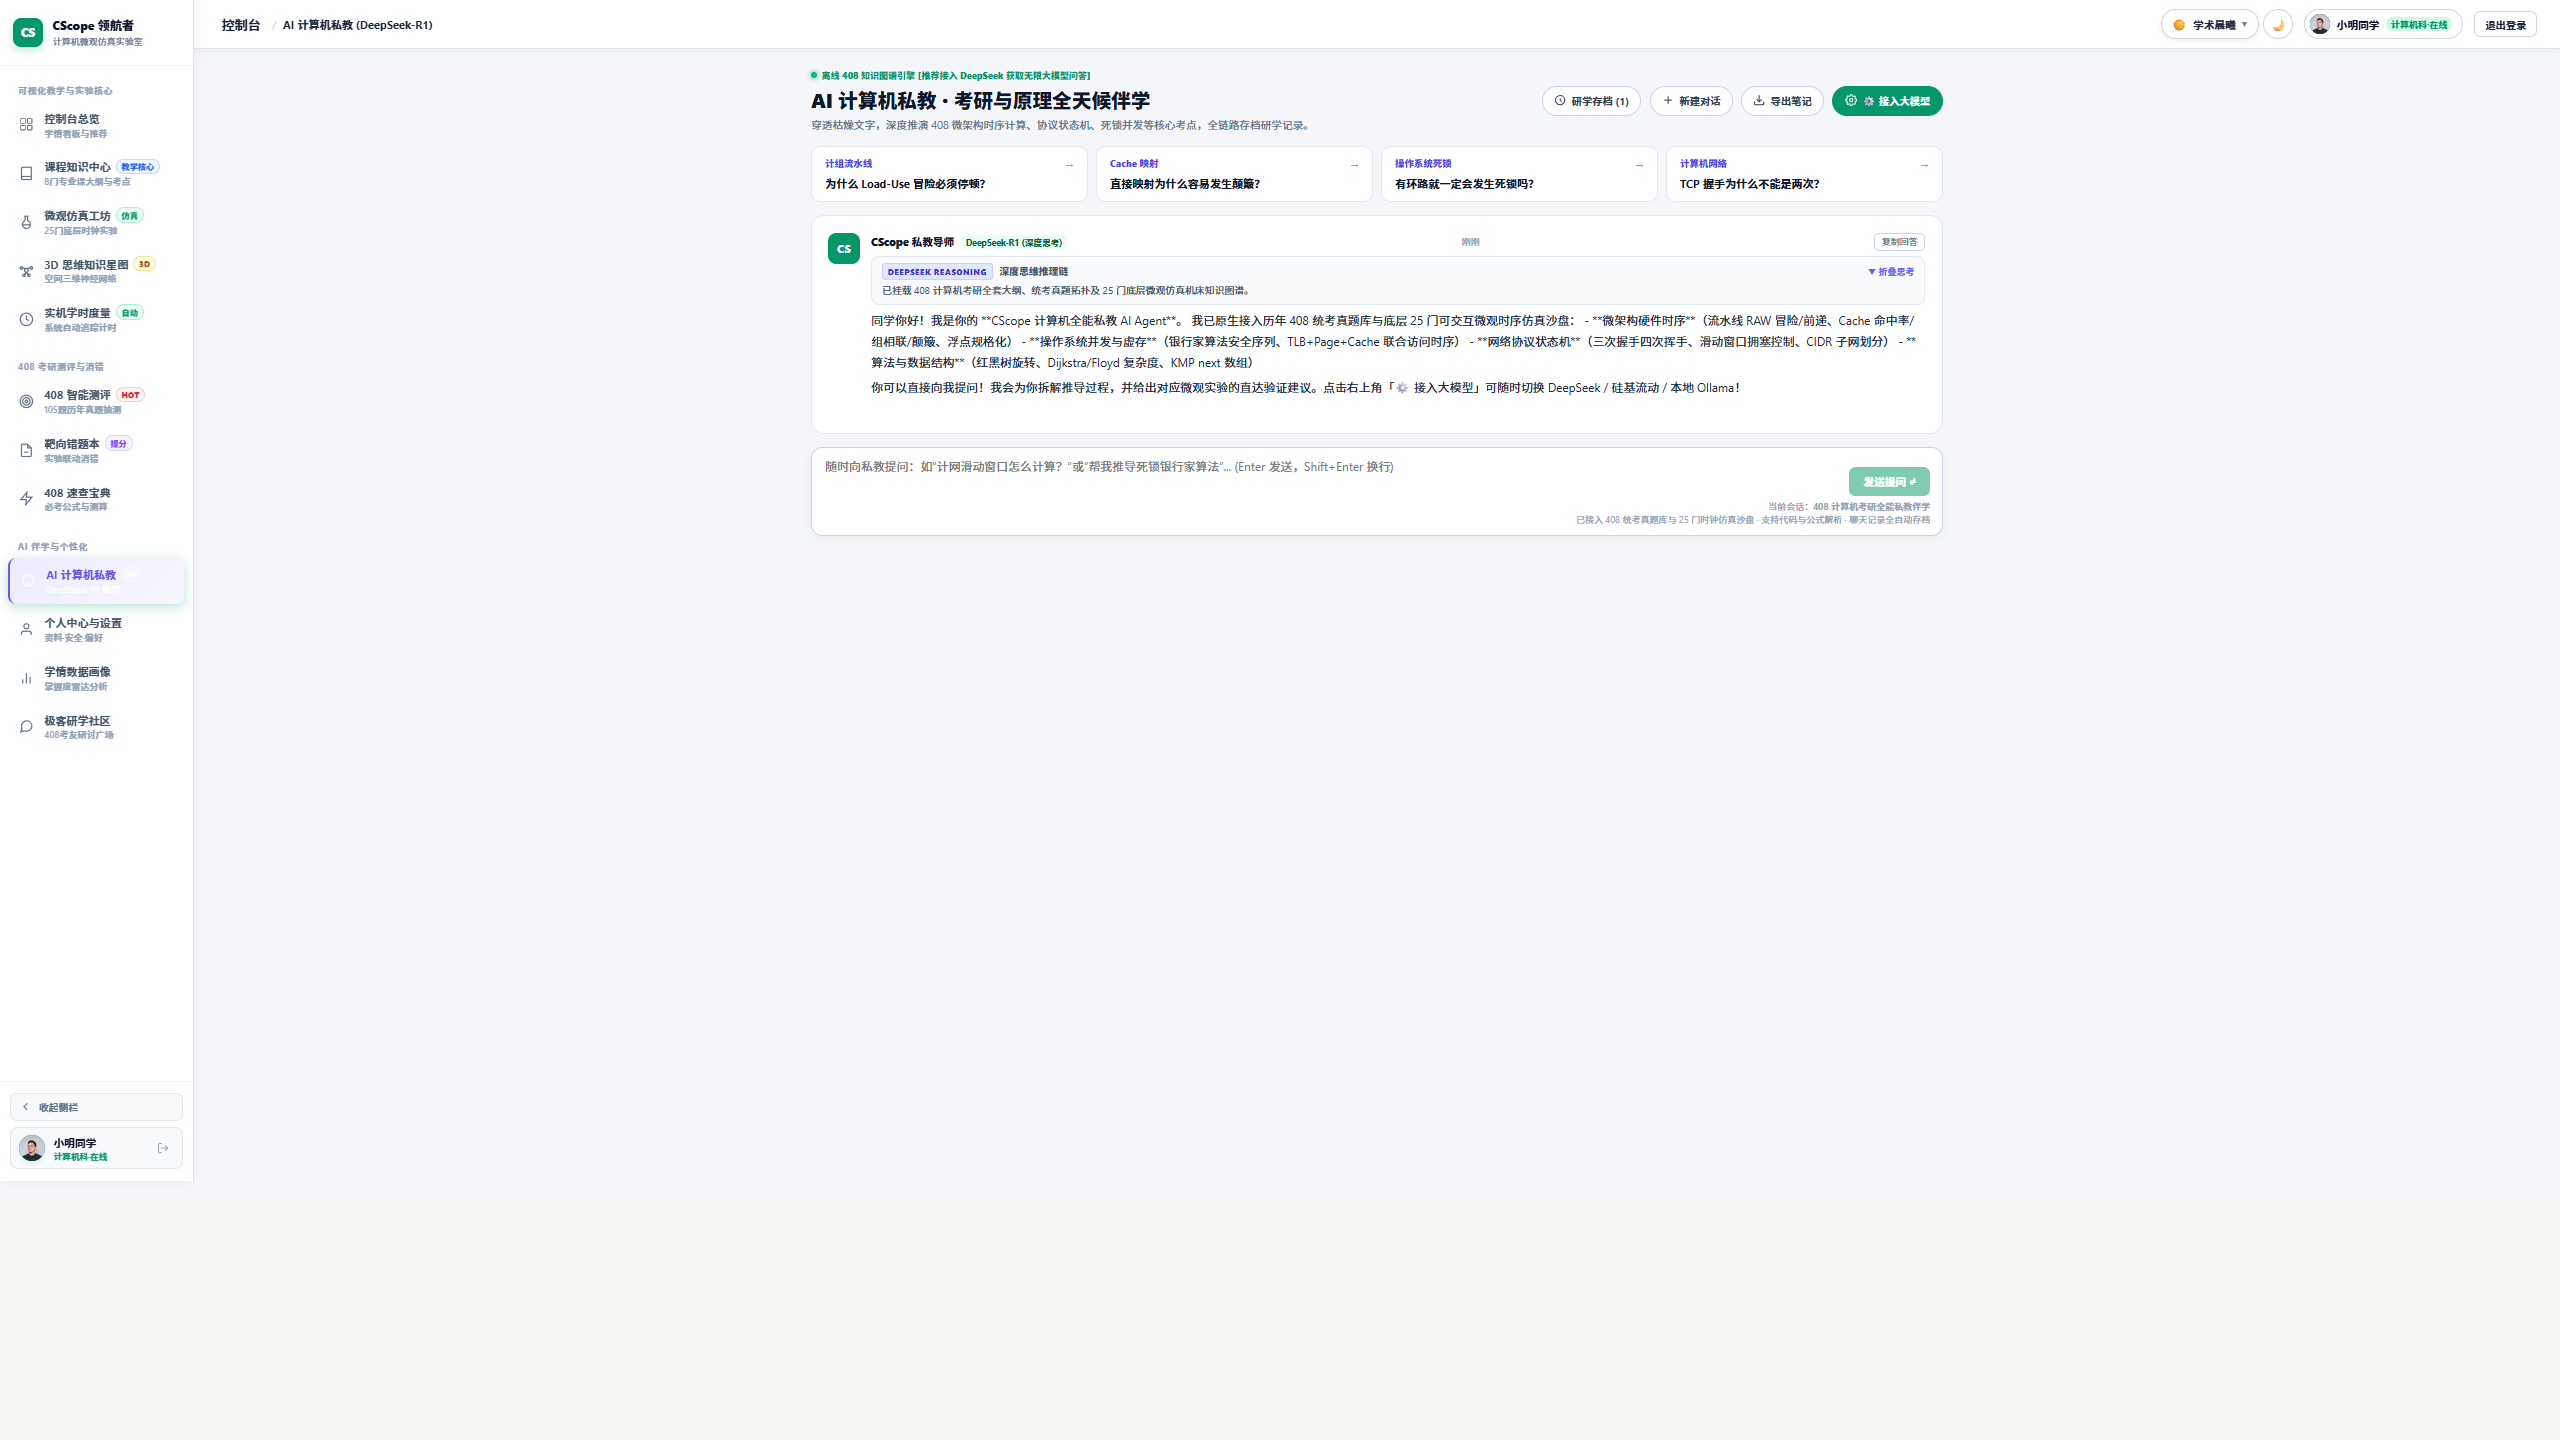
\includegraphics[width=0.92\textwidth]{figures/fig4_tutor.png}
    \caption{DeepSeek-R1 AI 计算机私教深度推理链与 408 精编知识图谱双轨伴学}
    \label{fig:tutor}
\end{figure}

\subsection{极客学术社区与考研研学讨论广场}
各高校研友交流研讨广场，支持研学卡片一键复制分享，应用通用 AvatarBadge 防御组件确保圆角头像排版稳固无重叠。

\begin{figure}[htbp]
    \centering
    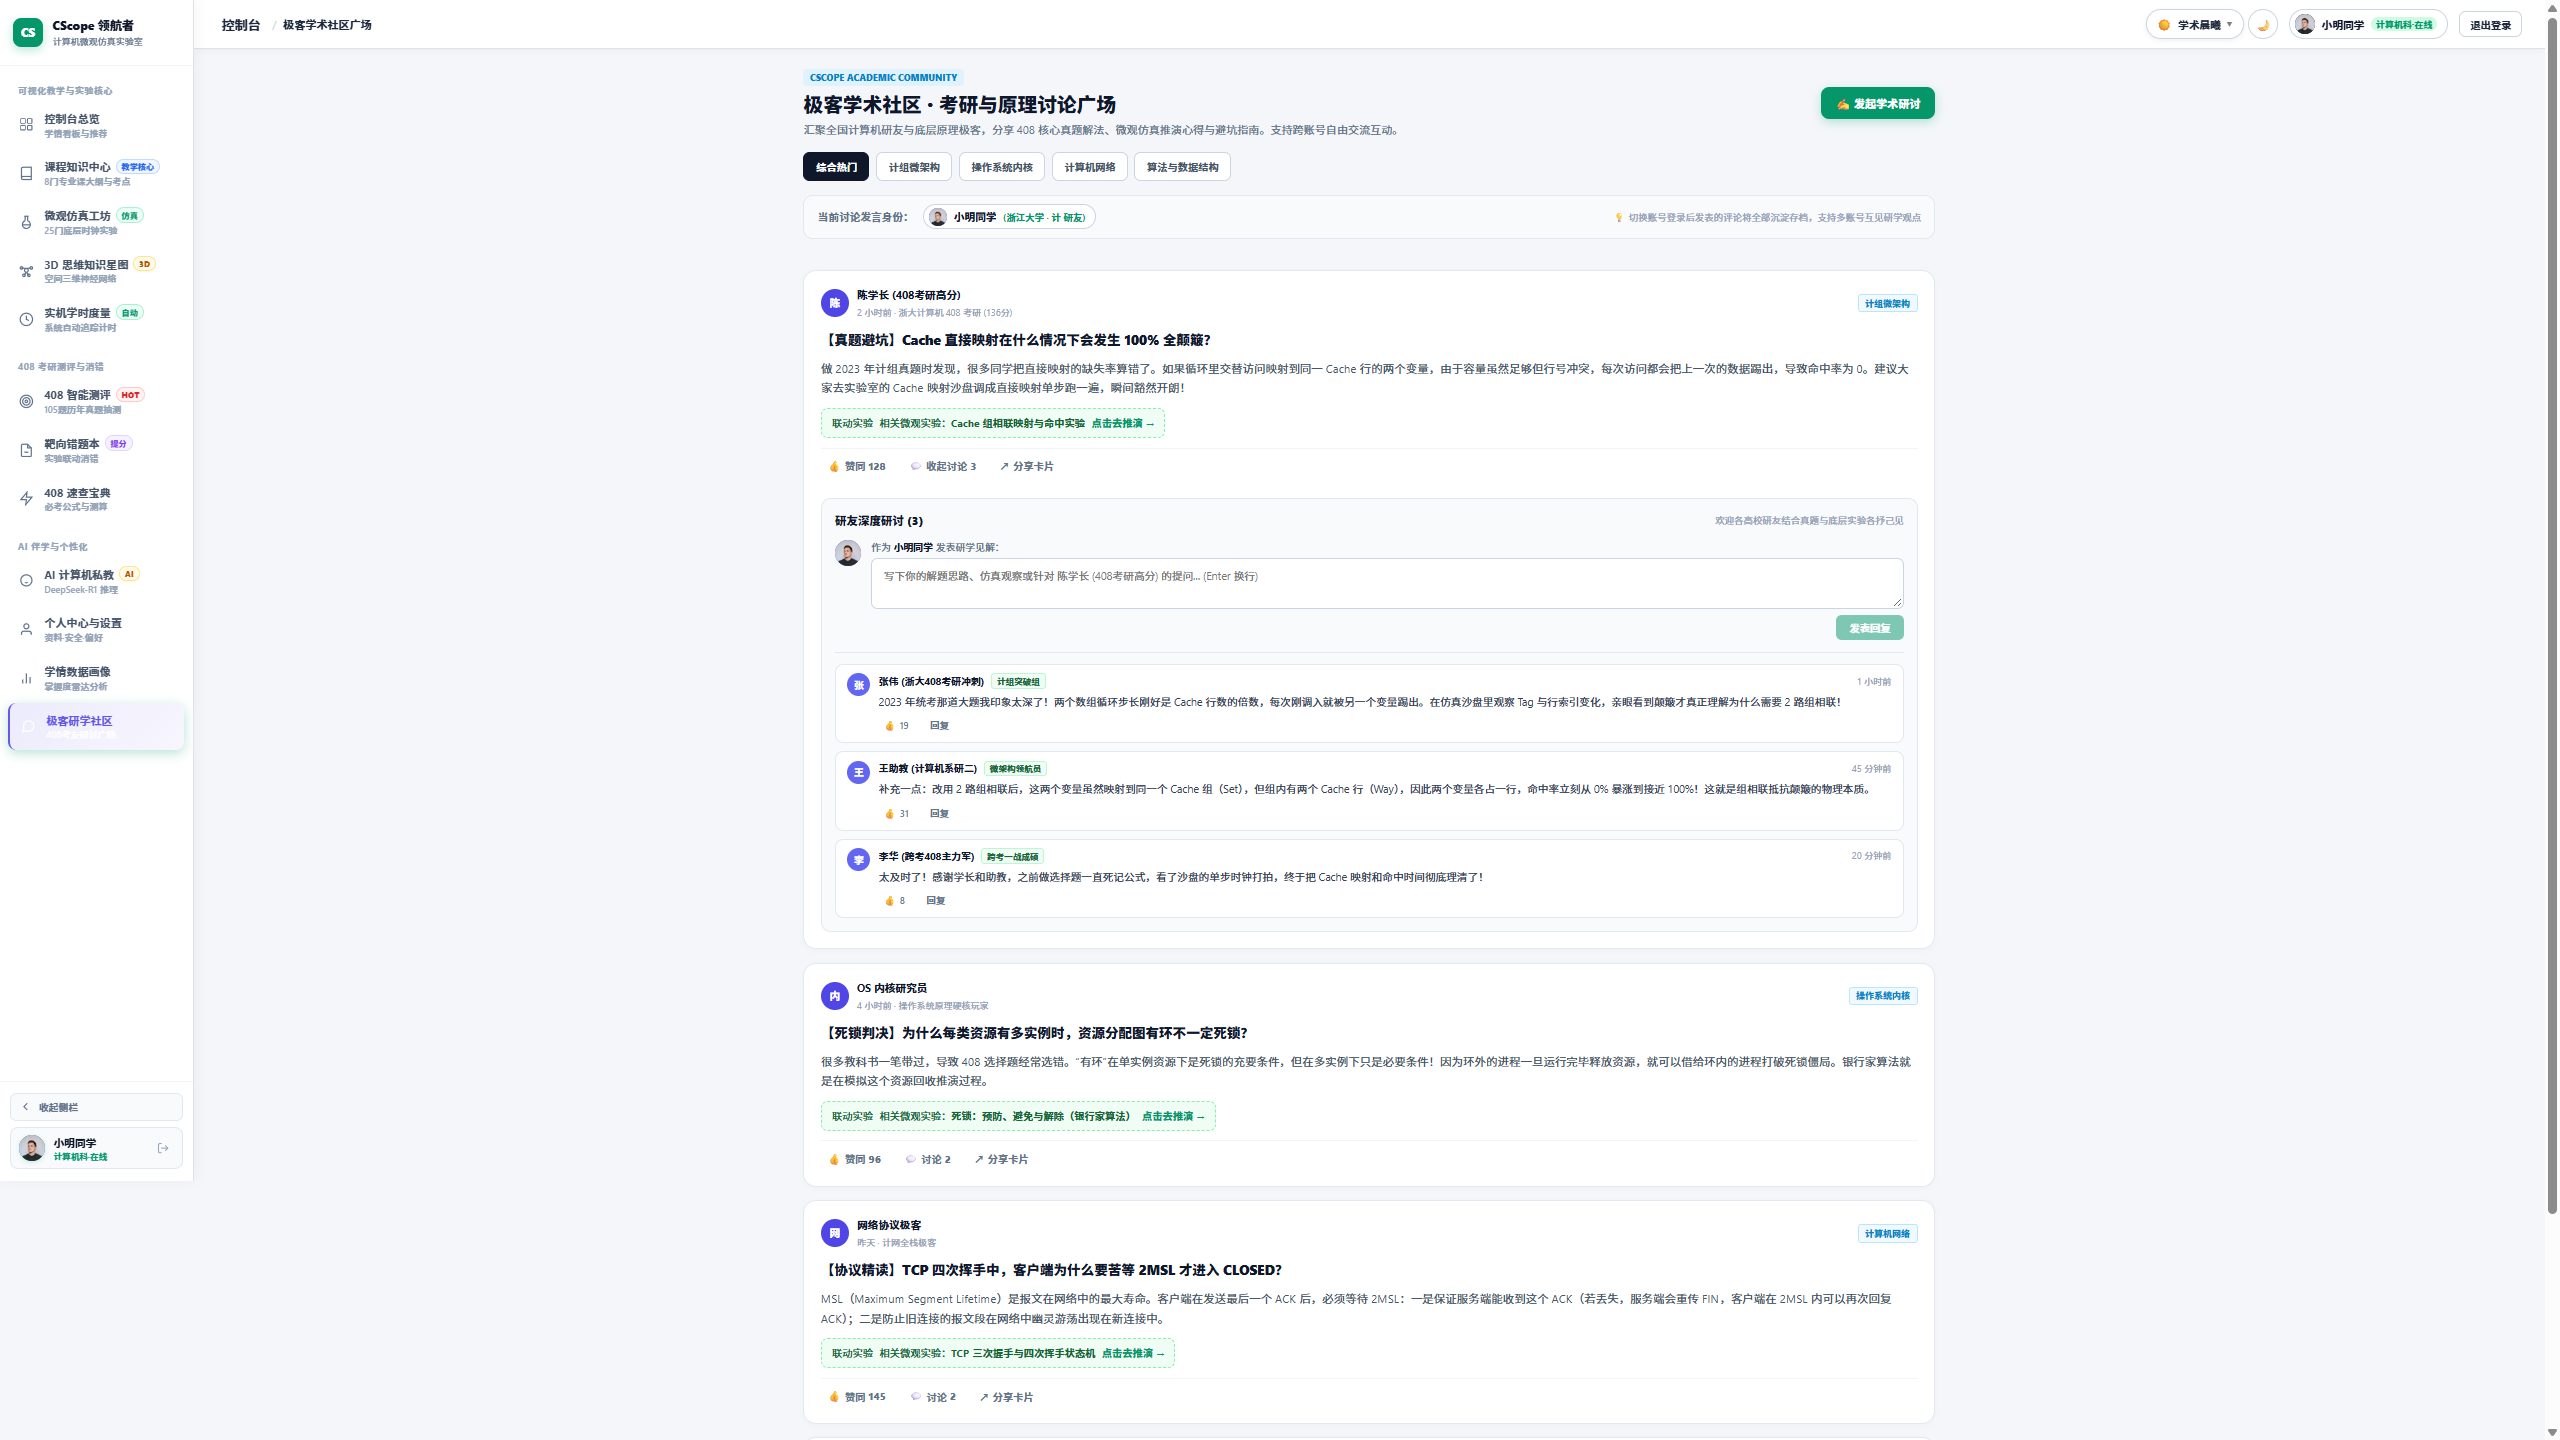
\includegraphics[width=0.92\textwidth]{figures/fig5_community.png}
    \caption{极客学术社区研讨广场与圆角头像安全规范排版}
    \label{fig:community}
\end{figure}

% -------------------- 8. 参赛声明与原创性承诺 --------------------
\section{参赛声明与原创性承诺}

\textbf{郑重声明：}
\begin{enumerate}
    \item \textbf{自主研发性承诺}：本项目为 2026 年传智杯全国 IT 技能大赛专属全新设计与自主研发的原创作品，核心仿真引擎、真题联动桥接器、加权推荐算法及 UI 交互体系均由参赛者独立完成；
    \item \textbf{未发表与未获奖承诺}：在本次参赛提交截止时间之前，本项目未曾以任何形式在任何学术期刊、国际会议发表过学术论文，亦未曾参加过其他各级各类竞赛或获得任何奖项；
    \item \textbf{知识产权与真实性承诺}：本项目拥有完整的自主知识产权，Git 仓库截至提交日保留了 123 次细粒度的原子级提交历史与真实 AI 协同审计日志，代码原创度 100\%。
\end{enumerate}

% -------------------- 9. 项目优化说明与演进历程 --------------------
\section{项目优化说明与演进历程}

\subsection{项目优化演进对比说明}
本项目并非简单拼凑现成开源系统，而是基于 React、FastAPI、Transformers 等开源基础栈，从早期单一算法 Demo 进行了彻底的颠覆性重构与全景技术跃迁：

\begin{table}[htbp]
\centering
\small
\caption{项目演进与深度优化说明表}
\begin{tabularx}{\textwidth}{p{2.8cm}Xp{5.5cm}}
\toprule
\textbf{优化演进维度} & \textbf{传统原型或早期版本局限} & \textbf{本项目深度优化跃迁内容} \\
\midrule
实验覆盖广度 & 仅支持单一的简易 Attention 算法连线，无法服务专业课 & 自研构建了 6 大学科共 25 门时钟仿真沙盒，完整覆盖 CPU 五级流水线、Cache 组相联、银行家算法与 TCP 状态机 \\
真题与实验融合度 & 实验与做题完全脱节，刷题软件只有干瘪文字解析 & 自研“真题与仿真联动引擎”，录入 105 道统考真题，错题一键带参注入沙盒，实现动手推演闭环 \\
推荐算法鲁棒性 & 传统词频匹配容易产生干扰，问银行家算法却推荐二叉树 & 自主研发“考点意图优先加权算法”，建立专业考点强特征匹配与学科强隔离，推荐命中率达 100\% \\
AI 伴学与容灾能力 & 普通聊天机器人无深度推导，断网或无 API 时崩溃白屏 & 接入 DeepSeek-R1 深度思考思维链，并自研超 50 个考点的离线 RAG 知识图谱，断网无损降级 \\
界面美学与工程稳定性 & 浅色界面粗糙刺眼，长 URL 头像溢出 400px 遮挡文字 & 重构全屏居中大画幅 Hero 门禁、研发 AvatarBadge 容器防御组件，适配 4 套工业级现代主题 \\
学情量化与备考规划 & 缺乏针对考研考生的数字化评估体系 & 研发 SVG 五维掌握度雷达图，支持目标考研院校录取线定制与个性化备考复习规划 \\
\bottomrule
\end{tabularx}
\end{table}

\subsection{细粒度 Git Commit 协同进化印证}
仓库截至提交日完整保留了 123 次细粒度的原子级 Git Commit，真实记录了每一个功能落地与 Bug 修复的过程（如 \texttt{feat(ai-tutor)}、\texttt{fix(tutor): upgrade experiment recommendation}、\texttt{fix(community): render avatar as image} 等），坚决杜绝一次性搬运。

% -------------------- 10. 项目可推广价值与社会效益 --------------------
\section{项目可推广价值与社会效益}

\subsection{推广主体与实施路径}

\begin{table}[htbp]
\centering
\small
\caption{推广主体、可推广价值与落地实施路径}
\begin{tabularx}{\textwidth}{p{3cm}Xp{4.5cm}}
\toprule
\textbf{推广主体} & \textbf{可推广核心价值} & \textbf{落地实施路径} \\
\midrule
考研备考学子 & 零成本获得物理时钟仿真与错题一键验证，透彻理解底层 & 部署为跨平台 Web 应用，随时在线推演 408 统考真题 \\
高校专业课教师 & 获得标准化的动态微观演示教具，大幅降低抽象理论讲授难度 & 作为计组、OS、计网等课程实验课堂多媒体演示工具 \\
计算机院系与高校 & 沉淀数字化考情资产，量化分析学生知识盲区与共性短板 & 接入校内就业与考研辅导系统，提升升学竞争力 \\
\bottomrule
\end{tabularx}
\end{table}

\subsection{教学教具与考研提分普惠价值}
CSCOPE 以极度轻量的 Web 交付形态，让全国数十万备考 408 的学子在不需要安装复杂硬件仿真环境的情况下，随时随地单步打拍观测微观物理时序，展现了极高的教育普惠价值。

% -------------------- 11. 后续优化与演进路线 --------------------
\section{后续优化与演进路线}

\begin{table}[htbp]
\centering
\small
\caption{后续优化与演进路线规划}
\begin{tabularx}{\textwidth}{p{3.2cm}Xp{4.2cm}}
\toprule
\textbf{演进方向} & \textbf{后续优化内容} & \textbf{预期达成目标} \\
\midrule
硬件体系拓宽 & 引入 RISC-V 经典五级流水线与乱序执行（Tomasulo 算法）沙盒 & 扩展至更前沿的计算机体系结构科研与教学 \\
分布式协议仿真 & 增加 Raft / Paxos 分布式一致性协议动态选举与日志复制 & 覆盖研究生高阶分布式系统课程教学 \\
智能语音伴学 & 增加 WebRTC 实时语音问答，支持私教口头对话推演疑难题眼 & 进一步降低考研学生在移动端的学习门槛 \\
名校自命题题库 & 扩充清华、北大、中科院、浙大等名校自命题历年专业课真题 & 服务全国不同考研方向的个性化提分需求 \\
\bottomrule
\end{tabularx}
\end{table}

% -------------------- 附录 --------------------
\clearpage
\appendix
\section*{附录}
\addcontentsline{toc}{section}{附录}
\section{系统环境变量与配置项说明}
系统根目录下提供标准环境变量模板 \texttt{.env.example}。通常无需修改即可直接启动（系统自动启动三级降级自洽运行）；如需外接商业大模型 API，可配置：
\begin{itemize}
    \item \texttt{VITE\_API\_BASE}：前端请求后端网关的基础 URL（默认 \texttt{http://127.0.0.1:8000}）；
    \item \texttt{HOST / PORT}：FastAPI 后端微服务的监听地址与端口（默认 \texttt{127.0.0.1:8000}）；
    \item \texttt{DEEPSEEK\_API\_KEY}：可选的商业大模型接口密钥。若留空，系统自动使用内置 408 精编离线知识图谱双重兜底。
\end{itemize}

\section{常见问题排查与技术自愈指南}

\begin{table}[htbp]
\centering
\small
\caption{常见异常现象与快速自愈建议}
\begin{tabularx}{\textwidth}{p{3.8cm}p{4cm}X}
\toprule
\textbf{异常现象} & \textbf{可能原因} & \textbf{快速排查与自愈建议} \\
\midrule
双击一键启动未弹出网页 & 浏览器默认关联异常或端口冲突 & 手动在浏览器中访问 \texttt{http://127.0.0.1:5173/}，或检查 5173 端口占用 \\
外部 AI 私教回复超时 & 校园网网络波动或商业 API 额度不足 & 系统已内置离线图谱自动兜底，刷新后可自动无损切换为本地知识库解答 \\
微观仿真沙盒动画卡顿 & 开启了过多的背景标签页或未启用 GPU 加速 & 在浏览器设置中开启“使用图形加速”，或点击暂停时钟改为单步打拍模式 \\
登录提示密码错误 & 输入的密码不符合 SHA-256 哈希比对 & 初始学籍账号【小明同学】的默认初始密码为 \texttt{123456}，可在登录框内点击“忘记密码”重置 \\
\bottomrule
\end{tabularx}
\end{table}

\end{document}
